\chapter{Modelling novel drug candidate dose response in influenza infection}
\label{ch:DARPin}

\dictum[Ann Leckie, "The Raven Tower"]{%
  One can make any number of careful and informed guesses, but until events occur any predictions are subject to error, to the extent that one's information, or one's understanding, may be incomplete. [...] The relevant question here, it seems to me, is not any of those things. It is, rather, Do you care?}%
\vskip 1em

Parts of this chapter were prepared during Pitt Meyer's 8-week research project "Modelling influenza A virus uncoating inhibition through host factor interaction" under Alina Artcibasova's supervision. Alina Artcibasova conceived the study, supervised the implementation of the mathematical model of DARPin-F10 mediated uncoating inhibition, and the analysis of the model predictions and parameter fitting. Alina Artcibasova performed literature data analysis, designed and implemented data-driven infection delay and  kinetic models, performed the fitting, prepared figures, and wrote the manuscript.

\section{Introduction}


In Chapter \ref{ch:ReactionModels} we have established that our "Symmetric" and "Asymmetric" HDAC6 complex formation models are capable of predicting capsid breakage in normal and perturbed conditions. Here we attempt to apply them to make predictions about perturbed conditions which require further mechanistic investigation. One possible application has been suggested by the data provided by our collaborators from Patrick Matthias' group at FMI. They investigated designed ankyrin repeat proteins (DARPins) - artificial proteins which can bind target proteins with high affinity and specificity - and found that DARPin-F10 inhibits HDAC6-mediated influenza uncoating. We used their experimental insight about DARPin-F10 together with our established HDAC6 complex formation models to make predictions about DARPin-F10 effective concentrations and dose response in HDAC6 mediated influenza uncoating.

To compare our dose-response predictions with experimental DARPin-F10 viral growth data we sought out existing influenza infection models. Non-structured \textit{in vitro} influenza kinetic models were considered a good fit for our goals, as they mostly rely on directly observed experimental quantities such as viral growth.

Some of the newer studies describing structured and non-structured kinetic models \cite{rudiger2019multiscale, schulze2009infection} use attractive multi-dimensional datasets, which even without the use of the model may allow predictions of infection progression. Such datasets, when available, provide an intriguing opportunity to functionally characterise influenza infection, and make corresponding adjustments in our model structure. For example, it has long been established that high multiplicity of infection (MOI) tends to lead to higher synchrony of viral release \cite{cairns1957asynchrony}. Influenza kinetic models tend to implicitly build such relationships into the parameter fitting. However, when the fitting dataset only includes a small variety of initial conditions, specifically with regard to initial virus concentration, it is difficult to judge how well the model would describe any other dataset.

In this chapter we give a brief summary of experimental data available for DARPin-F10 \cite{DarpinData} and provide an overview on \textit{in vitro} influenza kinetic modelling literature. We then model DARPin-F10 inhibition of HDAC6-Ub binding during influenza uncoating to predict active concentrations and dose-response behavior. We make use of available literature data \cite{rudiger2019multiscale, schulze2009infection} to analyze functional dependencies between model parameters, and to fit a simple influenza infection model, which we then use to predict the effect of DARPin-F10 on influenza infection.

\subsection{DARPin-F10 inhibits HDAC6-ZnF Ub binding}

\begin{figure}
\begin{center}
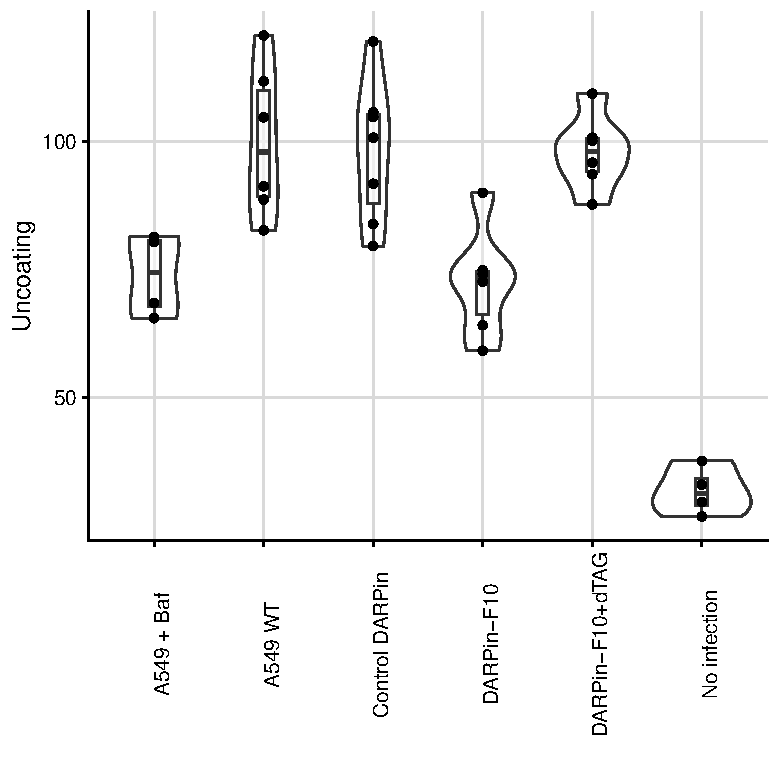
\includegraphics[width=0.95\textwidth, trim={0cm 0cm 0cm 0cm}, clip]{D_chapters/3_DARPinModels/DarpinUncoating.pdf}
\caption[DARPin-F10 reduces influenza virus uncoating]%
{DARPin-F10 at MOI = 30 PFU/ml reduces influenza virus uncoating\par
A549 + Baf: the cells treated with Bafilomycin, an ATPase inhibitor which also stops viral uncoating;\par
A549 WT: wild type;\par
CTR DARPin: cells with a DARPin that did not bind anything;\par
DARPin-F10: cells with a DARPin that binds HDAC6 ZnF;\par
DARPin-F10 + dTAG: cells in which DARPin F10 was degraded through dTAG before virus infection;\par
* No infection: cells without any virus added to them.\par
All the values are normalized to A549 WT.}
\label{figure:darpinUncoatingExperimental}
\end{center}
\end{figure}

\begin{figure}
\begin{center}
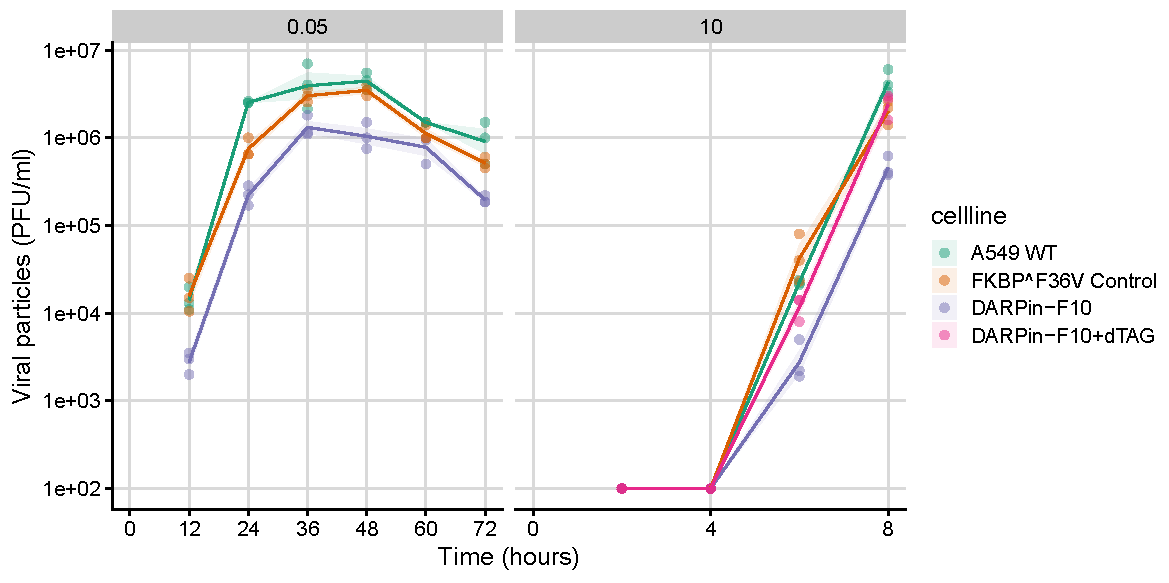
\includegraphics[width=0.95\textwidth, trim={0cm 0cm 0cm 0cm}, clip]{D_chapters/3_DARPinModels/DarpinVirusProduction.pdf}
\caption[DARPin-F10 reduces viral growth]%
{DARPin-F10 at MOI = 0.05 and 10 PFU/ml reduces viral growth\par
A549 WT: wild type;\par
FKBP\textasciicircum F36V Control: cell line with a different mutation.\par
DARPin-F10: cells with a DARPin that binds HDAC6 ZnF;\par
DARPin-F10 + dTAG: cells in which DARPin F10 was degraded through dTAG before virus infection.}
\label{figure:darpinGrowthExperimental}
\end{center}
\end{figure}

Our collaborators from Patrick Matthias’ group at FMI showed that DARPin-F10 has a high specificity and affinity against HDAC6-ZnF \cite{DarpinData}. They were able to stably express and degrade DARPin-F10 in A549 cells in inducable manner. Using these new mutant cell lines they demonstrated that expression of DARPin-F10 for MOI = 30 plaque-forming units (PFU)/ml leads to the reduction in influenza viral uncoating (Figure \ref{figure:darpinUncoatingExperimental}), and for MOI 10 and 0.05 PFU/ml - to a reduction in virus production (Figure \ref{figure:darpinGrowthExperimental}) by about an order of magnitude.

Knowing that DARPin-F10 binds to HDAC6-ZnF we can reasonably assume that during influenza uncoating it acts as a competitor against polyubiquitin chains. In this chapter, we use that assumption, and introduce DARPin-F10 to our HDAC6 complex formation models.

\subsection{Influenza infection modelling}

Seasonal and zoonotic influenza is a popular subject of viral modelling, which has a variety of approaches. The majority of viral models use systems of ordinary differential equations (ODE), but partial (PDE) and delay differential equations (DDE) have also been implemented.

Influenza infection dynamic models are focused primarily capturing the transmission between hosts, with the goal of informing public health decisions and assist in pandemic planning \cite{ferguson2006strategies, mcvernon2007model}.

With the advancement of social media, a new type of influenza forecasting models has emerged \cite{pawelek2014modeling, santillana2015combining, levy2018modeling}, relying on publicly available self-reporting by users.

Structured models which include individual processes in virus replication \cite{sidorenko2004structured}, endosomal escape \cite{lagache2012modeling} and defective viral particle propagation \cite{rudiger2019multiscale} have been proposed. Their phenomenological nature means that they often rely on unobserved quantities and variables, and do not allow for inference on specific molecular targets for intervention.

Non-structured influenza kinetic models aim to understand and quantify severity, duration, and overall progression of the infection within a host or a cell culture. \textit{In vitro} models rely on directly observed experimental quantities for parameter fitting. They usually have a simple and understandable structure. However this simplicity makes inference and analysis of specific molecular targets largely impossible. \textit{In vivo} kinetic models build up on that basic structure and attempt to incorporate innate \cite{beauchemin2008modeling, handel2010towards,miao2010quantifying} and adaptive \cite{belz2002compromised, handel2010towards, miao2010quantifying} immune response. Here we primarily focus on \textit{in vitro} models, as our DARPin-F10 experimental data is coming from cell culture experiments.

The chronic infection kinetic model, originally proposed for human immunodeficiency virus (HIV) \cite{perelson2002modelling}, includes three states: $T$ - target cells, $I$ - infected cells, $V$ - viral particles, which are described as a system of ODEs:

\begin{equation}
\begin{array}{rcl}
\frac{dT}{dt} &=& s T - d T - \beta T V \\
\frac{dI}{dt} &=& \beta T V - \delta I \\
\frac{dV}{dt} &=& p I - c V
\end{array}
\end{equation}

where $s$ is target cells regeneration, $d$ is natural target cells death, $\beta$ is target cells infection rate by viral particles, $\delta$ is death rate of infected cells, $p$ is viral particle production rate by infected cells, and $c$ is clearance rate of viral particles.

It is often assumed that during acute ($s = d = 0$ \cite{baccam2006kinetics}) influenza infection target cells $T$ are limited and are depleted over the course of the infection:

\begin{equation}
\begin{array}{rcl}
\frac{dT}{dt} &=& - \beta T V \\
\frac{dI}{dt} &=& \beta T V - \delta I \\
\frac{dV}{dt} &=& p I - c V
\end{array}
\end{equation}

Another commonly made assumption is that during influenza infection viral production is delayed, which is accomplished through presence of a latent eclipse phase infected cells $I_1$ and productively infected cells $I_2$ (\cite{baccam2006kinetics, smith2011effect}):

\begin{equation}
\begin{array}{rcl}
\frac{dT}{dt} &=& - \beta T V \\
\frac{dI_1}{dt} &=& \beta T V - k I_1 \\
\frac{dI_2}{dt} &=& k I_1 - \delta I_2 \\
\frac{dV}{dt} &=& p I_2 - c V
\end{array}
\end{equation}

where $k$ is a rate of $I_1$ maturation into $I_2$.

An alternative approach to modeling this latency is through the use of a system of delay differential equations (DDE), by introducing a fixed delay $\tau$:

\begin{equation}
\begin{array}{rcl}
&\frac{dT}{dt} = - \beta T(t) V(t) \\
&\frac{dI}{dt} = \beta T(t-\tau) V(t-\tau) - \delta I(t) \\
&\frac{dV}{dt} = p I(t) - c V(t)
\end{array}
\end{equation}

Here, during the "eclipse phase" the infected cell does not contribute to systems dynamics. A fixed delay model disregards variability of the transition time from eclipse phase, but allows to avoid unrealistically small or large transition times from the eclipse to productive phase \cite{beauchemin2008modeling}.

Models of viral production on microcarriers \cite{mohler2005mathematical,schulze2009infection} introduce a delay in the viral production term $p I(t - \tau)$ instead.

Several models have been suggested to describe influenza infection in presence of antiviral drugs. Amantadine drugs are commonly modelled as follows \cite{beauchemin2008modeling}:

\begin{equation}
\begin{array}{rcl}
\frac{dT}{dt} &=& - (1-\epsilon_{drug})\beta T V \\
\frac{dI}{dt} &=& \beta T V - \delta I \\
\frac{dV}{dt} &=& p I - c V
\end{array}
\end{equation}

where $\epsilon_{drug}$ is a drug efficacy, determined through a dose-response $E_{max}$ model:

\begin{equation}
\epsilon_{drug} = \epsilon_{max}\frac{1}{1 + (\frac{IC_{50}}{[D]})^{n}}
\end{equation}

where $\epsilon_{max}$ is a maximal drug effect such that $0 < \epsilon_{max} \le 1$, and $n \ge 0$ is a Hill coefficient.

In an alternative formulation, amantadine lengthens the eclipse phase instead of inhibiting the infection \cite{beauchemin2008modeling}:

\begin{equation}
\begin{array}{rcl}
\frac{dT}{dt} &=& - \beta T V \\
\frac{dI_1}{dt} &=& \beta T V - (1-\epsilon_{drug}) k I_1 \\
\frac{dI_2}{dt} &=& (1-\epsilon_{drug}) k I_1 - \delta I_2 \\
\frac{dV}{dt} &=& p I_2 - c V
\end{array}
\end{equation}

Similarly, neuraminidase inhibitors are often assumed to influence viral production rate $(1-\epsilon_{drug}) p I$ instead \cite{handel2007neuraminidase}.

\section{Results}

To simulate the inhibition of HDAC6-mediated uncoating by DARPin-F10 we created two new HDAC6 complex formation models: "Symmetric DARPin" and "Asymmetric DARPin" (Figure \ref{figure:darpinReactionModelSchemes}, see Appendix \ref{appendix:DARPinModelsEquations} for details) based respectively on "Symmetric" and "Asymmetric" model variants, as reported in Chapter \ref{ch:ReactionModels}. The key difference between them follows from the structure of the original models. Ub only assists the binding of myosin in the "Asymmetric" model, so the presence of DARPin-F10 would only inhibit myosin recruitment, while for the "Symmetric" model DARPin-F10 would affect the recruitment of both myosin and dynein motors.

\begin{figure}
\begin{center}
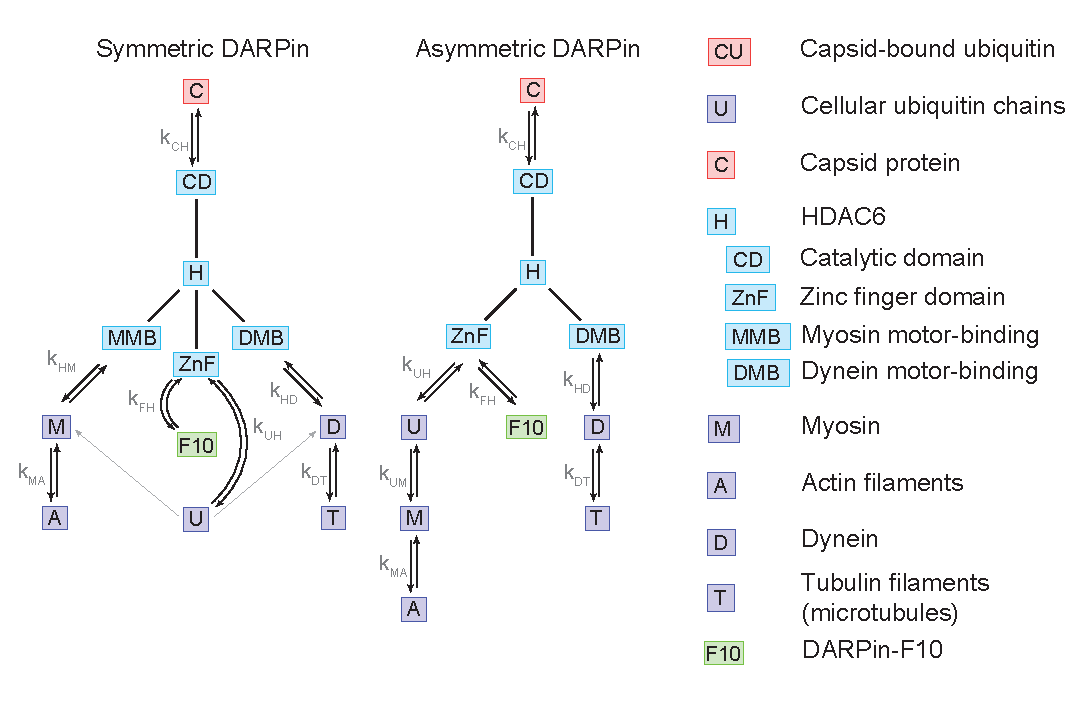
\includegraphics[width=0.95\textwidth, trim={0cm 0cm 0cm 0cm}, clip]{D_chapters/3_DARPinModels/ReactionModelSchemesDarpin.pdf}
\caption[HDAC6 complex formation models densities with and without DARPin-F10]%
{Interaction schematics for the two DARPin-F10 reaction model variants. Nodes represent proteins or protein domains (linked by solid lines) and arrows denote biochemical reactions with corresponding on-rates indicated next to the arrows. Node colors distinguish between viral proteins (red), HDAC6 (cyan), other host proteins (purple), and DARPin-F10 (green).}
\label{figure:darpinReactionModelSchemes}
\end{center}
\end{figure}

\begin{figure}
\begin{center}
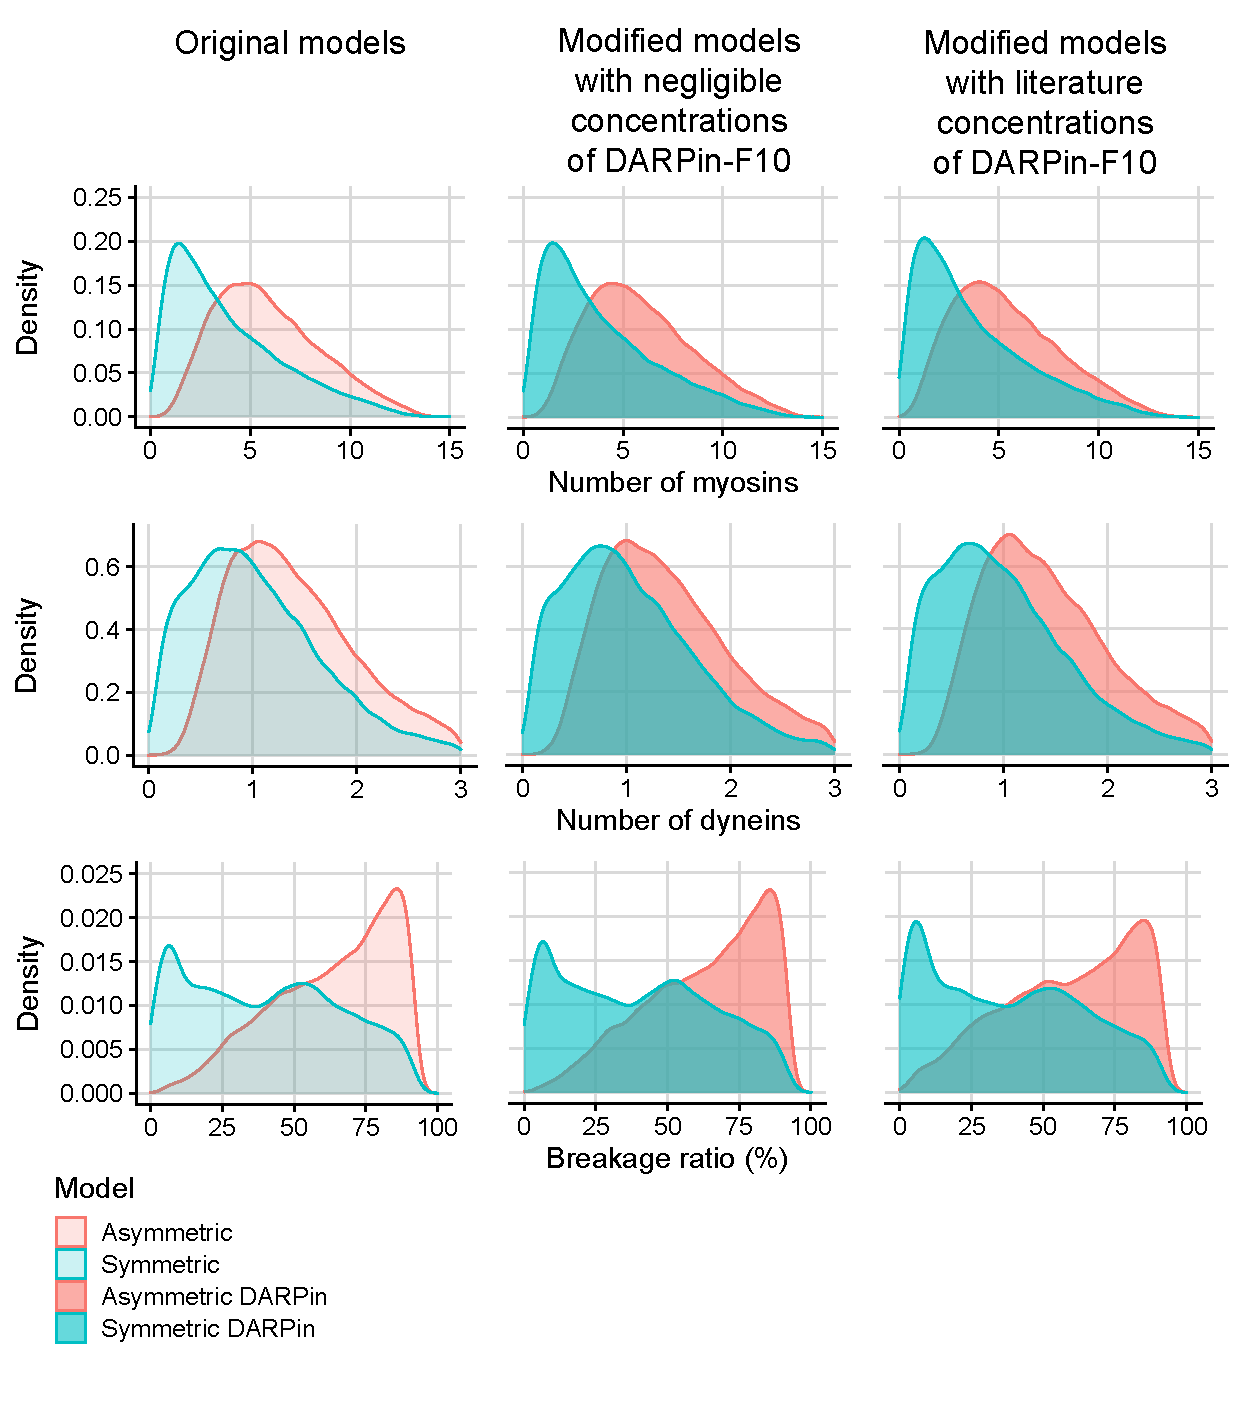
\includegraphics[width=0.95\textwidth, trim={0cm 0cm 0cm 0cm}, clip]{D_chapters/3_DARPinModels/Density_DARPin.pdf}
\caption[HDAC6 complex formation models densities with and without DARPin-F10]%
{HDAC6 complex formation models densities with and without DARPin-F10.\par
Arrows are aligned to highlight the change in the density between the original model and the modified DARPin-F10 model.}
\label{figure:darpinDensities}
\end{center}
\end{figure}

To verify that the base reaction network of our modified HDAC6 models functions as before, we uniformly sampled reactions and rates around our starting point for two concentrations of DARPin-F10 - one negligibly small, and $34.7$ nM - value compatible with DARPin concentrations previously reported in literature \cite{guillard2017structural} (Figure \ref{figure:darpinDensities}, see Methods \ref{ch:DARPinMethods} for detail). Modified models with negligible concentrations of DARPin-F10 performed largely the same as before. While the difference in densities for DARPin-F10 for literature reported concentrations is mild, it is clear that for the modified "Asymmetric DARPin" model the peak of myosin recruitment is shifted slightly from 5 to 4 compared to the original model. Likewise, the modified "Symmetric DARPin" model on average recruits slightly fewer dyneins than the original model. These changes in motor recruitment lead to a density increase in the low capsid breakage ratio for the "Symmetric DARPin" model and a density decrease of high capsid breakage ratio for the "Asymmetric DARPin" model (Figure \ref{figure:darpinDensities}).

\begin{figure}
\begin{center}
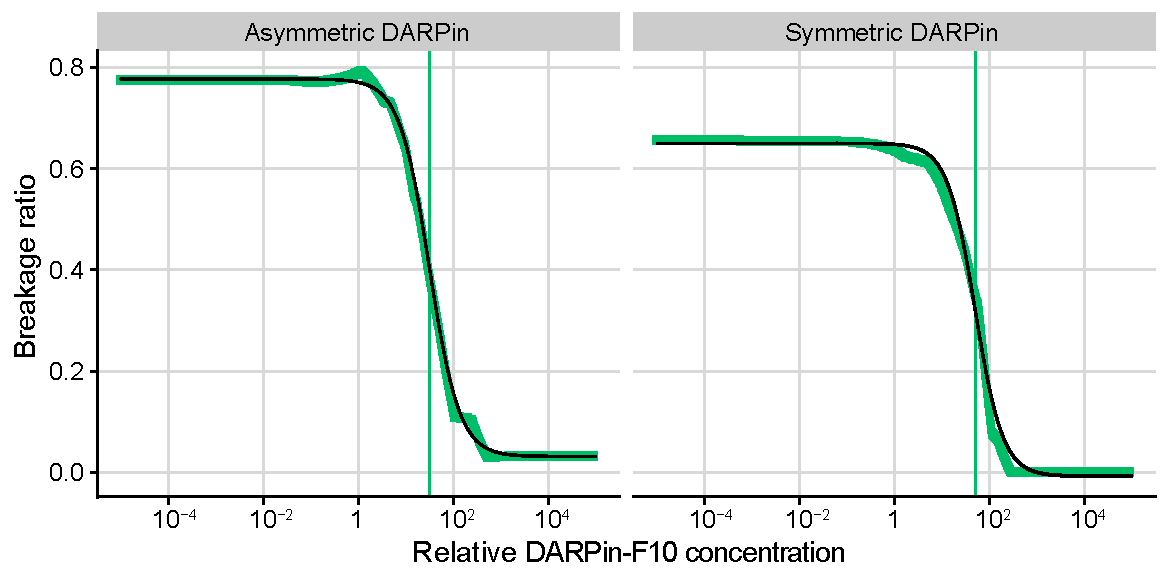
\includegraphics[width=0.95\textwidth, trim={0cm 0cm 0cm 0cm}, clip]{D_chapters/3_DARPinModels/FitDarpinTrajectories.pdf}
\caption[Capsid breakage prediction depending on relative DARPin-F10concentration]%
{Capsid breakage prediction depending on relative DARPin-F10 concentration. \par
The green trajectory is a direct prediction from the model, the black line is a corresponding Hill equation fit. All the concentrations are relative to literature value $34.7$ nM, corresponding to 1 on the plot. The vertical green line denotes EC50 value of the fit.}
\label{figure:darpinTrajectories}
\end{center}
\end{figure}

To simulate influenza uncoating dose response to DARPin-F10 we widely sampled the DARPin-F10 concentration near the literature value, and ran simulations for both "Symmetric DARPin" and "Asymmetric DARPin" models of HDAC6 complex formation. Both models displayed similar sigmoidal behavior for DARPin-F10 (Figure \ref{figure:darpinTrajectories}). At low concentrations the breakage ratio for both models stayed approximately the same as before (Figure \ref{figure:sampledTrajectories}), with the "Asymmetric DARPin" model variant achieving higher capsid breakage. Increasing DARPin-F10 concentration lead to a dramatic drop in the observed capsid breakage ratio.

To characterize resulting trajectories we fitted them using the Hill equation for dose response (Figure \ref{figure:darpinTrajectories}). Notably, "Asymmetric DARPin" had a lower half maximal effective concentration at approximately 1.1 $\mu$M, compared to "Symmetric DARPin" at approximately 1.7 $\mu$M.

To estimate effective DARPin-F10 concentrations, we used our Hill equation fits with estimates of DARPin-F10 efficiency we obtained from the experimental data provided by our collaborators \cite{DarpinData} (Table \ref{table:DARPinFittingCoefficients}). For the uncoating assays the effective DARPin-F10 concentrations for both model variants ended up slightly under 1 $\mu$M. For viral growth curves they were approximately 2.5 $\mu$M for MOI = 0.05 PFU/ml, and 7 $\mu$M for MOI = 10 PFU/ml. These concentrations are significantly higher than our starting DARPin-F10 concentration of $34.7$ nM or cellular HDAC6 concentrations, but are not outside of bounds for intracellular protein expression \cite{milo_2015}.  \cite{guillard2017structural} uses biochemical assays with DARPin concentrations at 3 $\mu$M to characterise their binding kinetics.

\subsection{Influenza delay as a function of MOI}

Influenza kinetic models often rely on available datasets for parameter fitting. This often leads to a variety of implicit assumptions about the infection, for example, that delay time $\tau$ in delay models is constant across the variety of MOIs. It is, however, well known that higher MOI usually leads to higher synchrony \cite{cairns1957asynchrony}, and earlier observed onset of infection, in the form of an earlier start of viral production.

\begin{figure}
\begin{center}
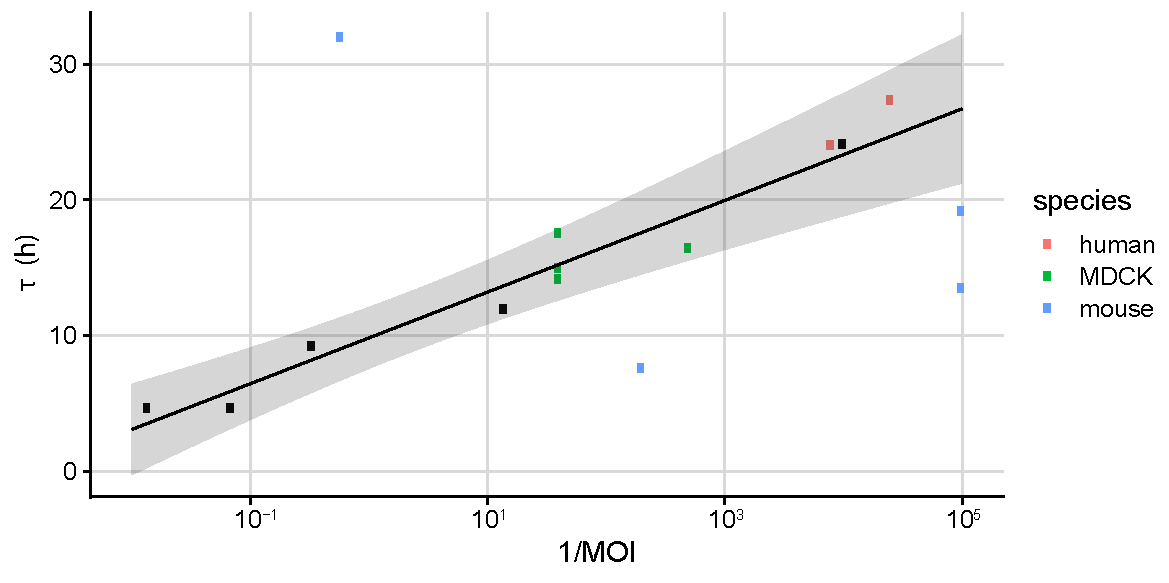
\includegraphics[width=0.95\textwidth, trim={0cm 0cm 0cm 0cm}, clip]{D_chapters/3_DARPinModels/DelayMoiValidation.pdf}
\caption[Influenza virus infection delay as a function of initial MOI]%
{Influenza virus infection delay as a function of initial MOI. \par
Black datapoints correspond to \cite{frensing2016influenza, rudiger2019multiscale, DarpinData} data used to fit the model. Red, green, and blue points correspond to the data calculated based on the delay times estimated from other publications, and the corresponding MOI.}
\label{figure:delayMoiValidation}
\end{center}
\end{figure}

To analyze the dependency between $\tau$ and MOI (Figure \ref{figure:delayMoiValidation}) we use an available literature dataset \cite{frensing2016influenza, rudiger2019multiscale} which reports influenza virus production for three values of MOI = $73$, $3$, $10^{-4}$, and WT measurements in our collaborators DARPin-F10 data \cite{DarpinData}.

Observed delay times were calculated based on an asymptotic regression function, fitted on the viral production data. Based on experimental observations, we used considerations that the dependency must have inverse proportionality to MOI, and that based on the observed delay values it is at least logarithmic. We fitted the resulting relationship between delay time $\tau$ and MOI:

\begin{equation}
\tau = a + b \log_e \Big(\frac{1}{MOI}\Big)
\label{eq:delayMOI}
\end{equation}

where $a$ = 9.83 is the delay for MOI = 1, and $b$ = 1.47 is the slope coefficient. It is worth to note that MOI = 1 has a special meaning corresponding to number of viral particles being equal to the number of target cells, making it a characteristic point for this expression.

The relationship in Equation \ref{eq:delayMOI} would break down at the very high values of MOI, both due to mathematical limitation - at $\tau$ turning negative, and biological considerations - no matter how much virus we add to the system, there will always be lag time due to internalization and uncoating processes within the cell. However, in practice, such high MOI values are used in experiments relatively rarely, and even MOI = 73 is an extreme.

Our validation using other experimental data shows that human and Madin-Darby canine kidney (MDCK) cell culture data fit our delay-MOI relationship quite well, while mice results disagree. This discrepancy may be explained by the difficulty of measuring the exact amounts of virus inhaled during the experiment by the mouse. However, in both human and mice experiments the number of observed data points is not very high, so their predictive power may vary.

\subsection{Characterising the fraction of infectious virus production}

During influenza infection viruses often produce virions which do not carry the full set of vRNPs, or are damaged in some other way. Those faulty viral particles are called defective interfering particles (DIPs). Their ability to infect and propagate relies on coinfection with fully infectious viral particles, but coinfected cells tend to release primarily progeny DIPs \cite{frensing2014impact}. At high MOI values most cells are infected with several virions, providing the best conditions for DIP accumulation. Thus, another quantity of interest is infectious fraction - the fraction of infectious viral particles compared to total viral particles produced during the infection:

\begin{equation}
    \text{Infectious fraction} = \frac{\text{Number of infectious virions}}{\text{Total number of virions}}
\end{equation}

\begin{figure}
\begin{center}
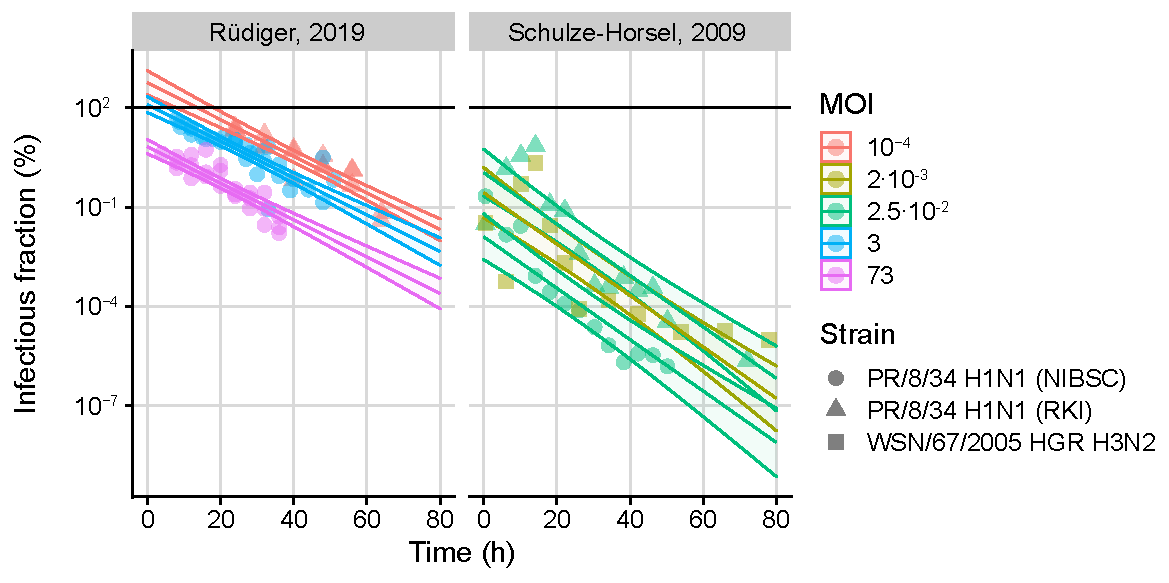
\includegraphics[width=0.95\textwidth, trim={0cm 0cm 0cm 0cm}, clip]{D_chapters/3_DARPinModels/InfectiousFractionAll.pdf}
\caption[Infectious fraction of virus production over the course of infection]%
{Infectious fraction of virus production over the course of infection for 3 different strains and 5 values of MOI, based on the data from \cite{frensing2016influenza, rudiger2019multiscale} and digitalized data from \cite{schulze2009infection}. Each panel has been fitted as a parallel slope model, R\"udiger, 2019 \cite{rudiger2019multiscale} based on MOI, and Schulze-Horsel, 2009 \cite{schulze2009infection} based on the strain used.}
\label{figure:infectiousFraction}
\end{center}
\end{figure}

A simple plot of infectious fraction \cite{rudiger2019multiscale, frensing2016influenza} as a function of time after infection reveals a linear relationship between the two, offset by the MOI value (Figure \ref{figure:infectiousFraction}, left). Unfortunately, with just 3 data points we can only observe that in accordance with our expectations high MOI leads to a low infectious fraction, but this relationship may be confounded by the use of two different viral strains.

Another study \cite{schulze2009infection} uses the same two strains, along with one H3N2 strain, at two different values of MOI, so we used their digitized data to plot the infectious fraction, hoping for an additional insight. Regardless of specific strain and MOI used, infectious fraction still displays a similar log-linear relationship with time. However, it is apparent that the overall infectious fraction is lower than what was observed in \cite{rudiger2019multiscale, frensing2016influenza} by about 3 orders of magnitude, despite the fact that the MOI values used by \cite{schulze2009infection} are relatively low. Whether that is due to their use of microcarrier culture, or simply an artifact of preparation is unclear.

Unfortunately, these discrepancies in experimental data do not allow us to make quantitative predictions about the relationship between infectious fraction, MOI, and viral strains, but they present an interesting case for future research efforts.

\subsection{Influenza infection model selection}

Literature dataset \cite{rudiger2019multiscale} displayed a slow depletion of target cells over the course of infection, prompting us to consider chronic models and models with a target cell population described by a fitted Hill equation. For chronic models the target cell population is slowly renewed over the course of infection with a constant rate $g$. For models with a target cell population described by a fitted Hill equation, the infection is limited by target cell availability later in the infection:

\begin{equation}
T = \frac{T_0}{1+\exp \big(n^{Target}\log_e(\frac{EC_{50}^{Target}}{T})\big)}
\end{equation}

where $T$ is the current number of target cells, $T_0$ is the initial number of target cells, $EC_{50}^{Target}$ is a half maximal effective concentration of target cells, $n^{Target}$ is a Hill coefficient of target depletion.

To model influenza virus infection, we prepared two chronic and seven depletion infection models, which we named after the states and parameters they include (Figure \ref{figure:compartamentalSchematic}, Appendix \ref{appendix:compartmentalModelEquations}). We fitted these models (Table \ref{table:ModelObjFunction}) using literature data \cite{rudiger2019multiscale, frensing2016influenza} for three values of MOI. Judging by the objective function values, as well as visual evaluation of the fits (Appendix \ref{appendix:compartmentalModelFits}), models with a target cell population described by a fitted Hill equation performed the best, reaching objective function values about an order of magnitude lower than the next candidates (Table \ref{table:ModelObjFunction}). In the following analysis we only focus on these three models.

\begin{figure}
\begin{center}
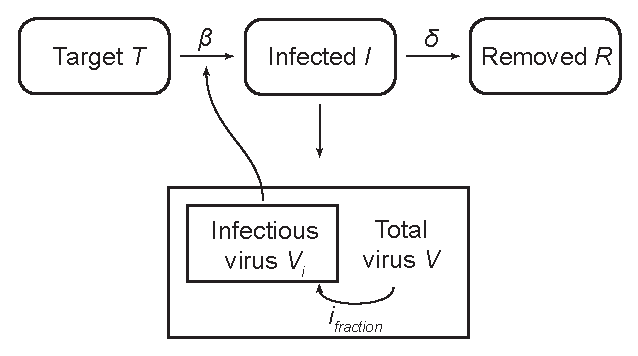
\includegraphics[width=0.95\textwidth, trim={0cm 0cm 0cm 0cm}, clip]{D_chapters/3_DARPinModels/compartamentalSchematic.pdf}
\caption[Schematic representation of a simple TIRVV$_i$ kinetic model]{Schematic representation of a simple TIRVV$_i$ kinetic model \par
Rectangles represent virus populations, and rounded rectangles represent cell populations. Arrows indicate transitions between populations.}
\label{figure:compartamentalSchematic}
\end{center}
\end{figure}

\newpage

\begin{figure}[H]
\begin{center}
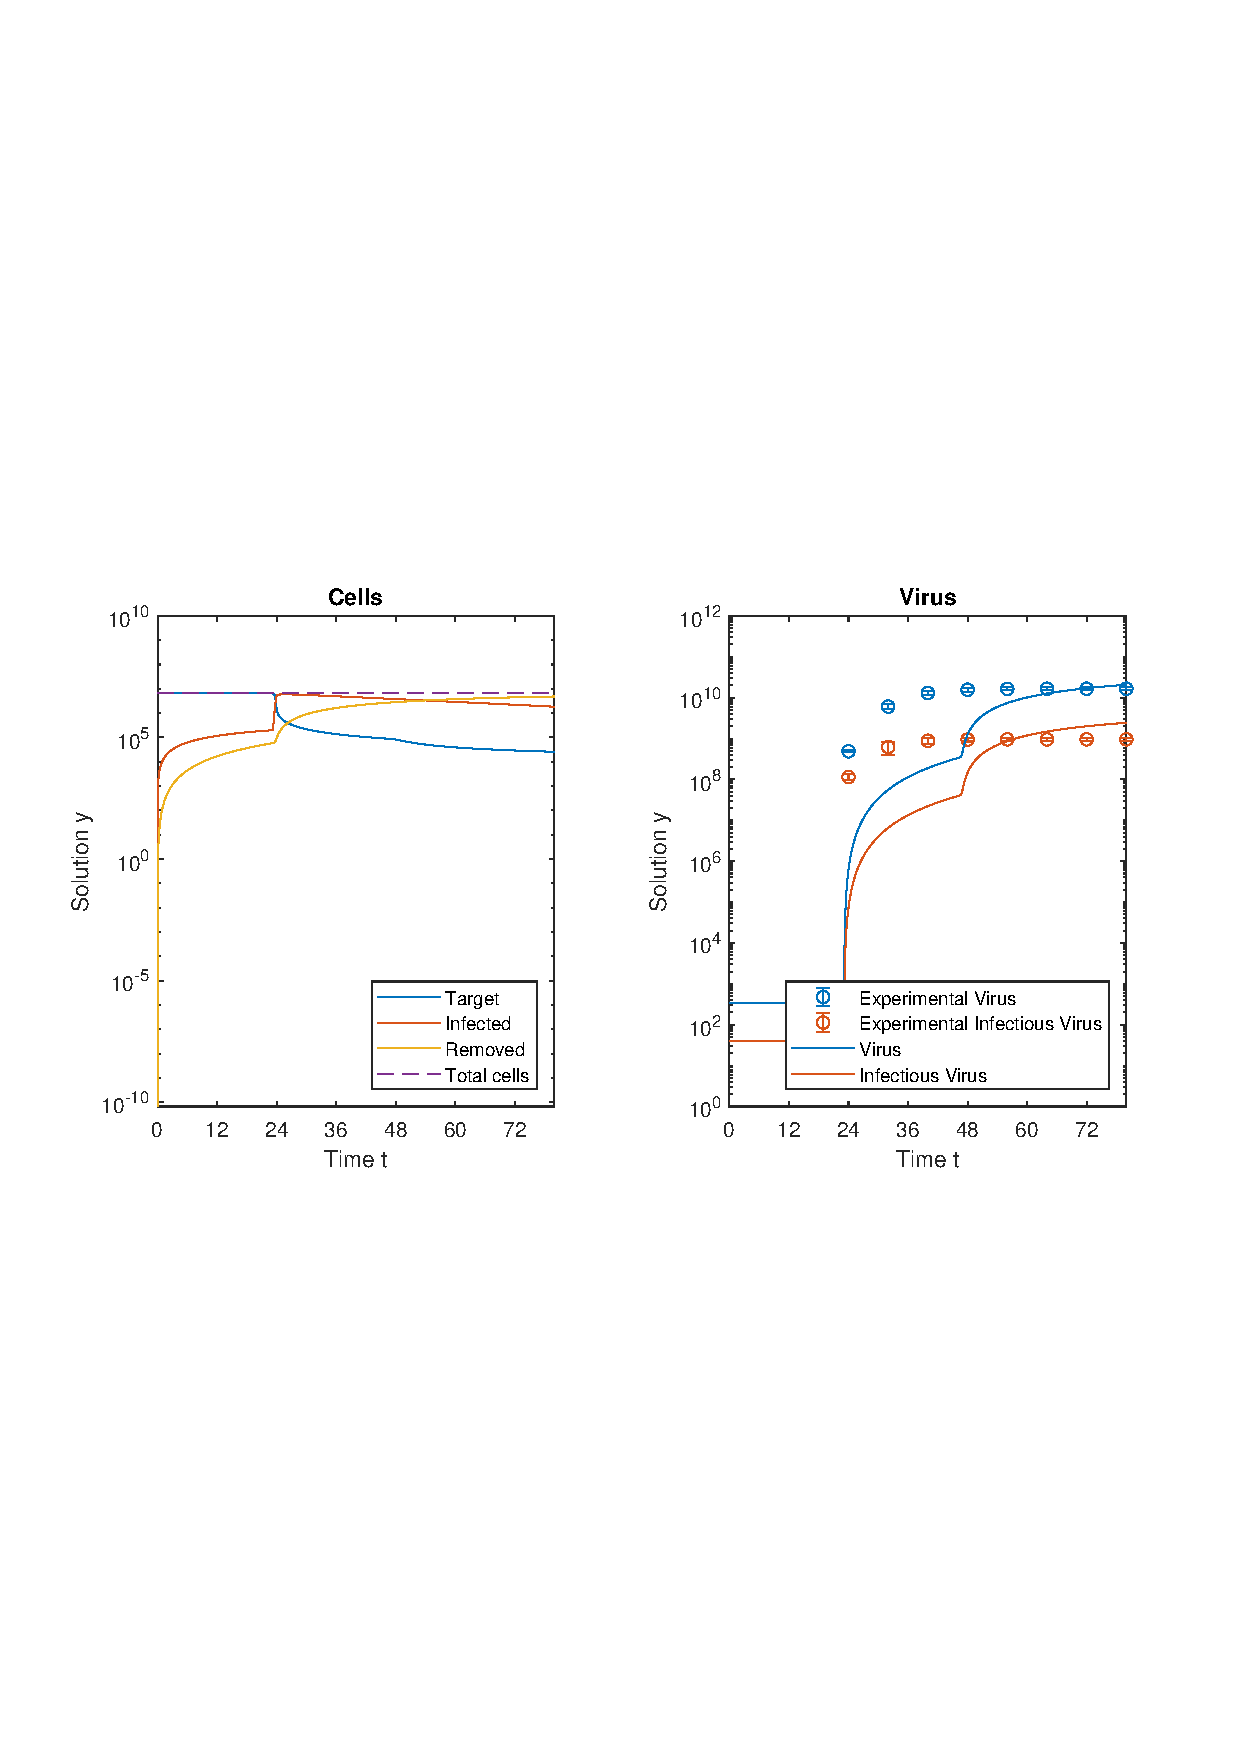
\includegraphics[width=0.6\textwidth, trim={1cm 9.5cm 1cm 9.5cm}, clip]{D_chapters/6_appendix/4_THillIRVViDelay/ModelTHillIRVViDelayDSNSaenz2010FittedMOI0.0001B0.0010133D0.55548P3247.2256C0.0027335TIC1896440.1965TH4.9813iFrac0.11736log.pdf}
\caption[T$_{Hill}$IRVV$_i$, delay $\tau = f(\text{MOI})$ model fit for MOI = $10^{-4}$]%
{T$_{Hill}$IRVV$_i$, delay $\tau = f(\text{MOI})$ model fit for MOI = $10^{-4}$}
\label{figure:THillIRVViDelayMOI00001}
\end{center}
\end{figure}

\begin{figure}[H]
\begin{center}
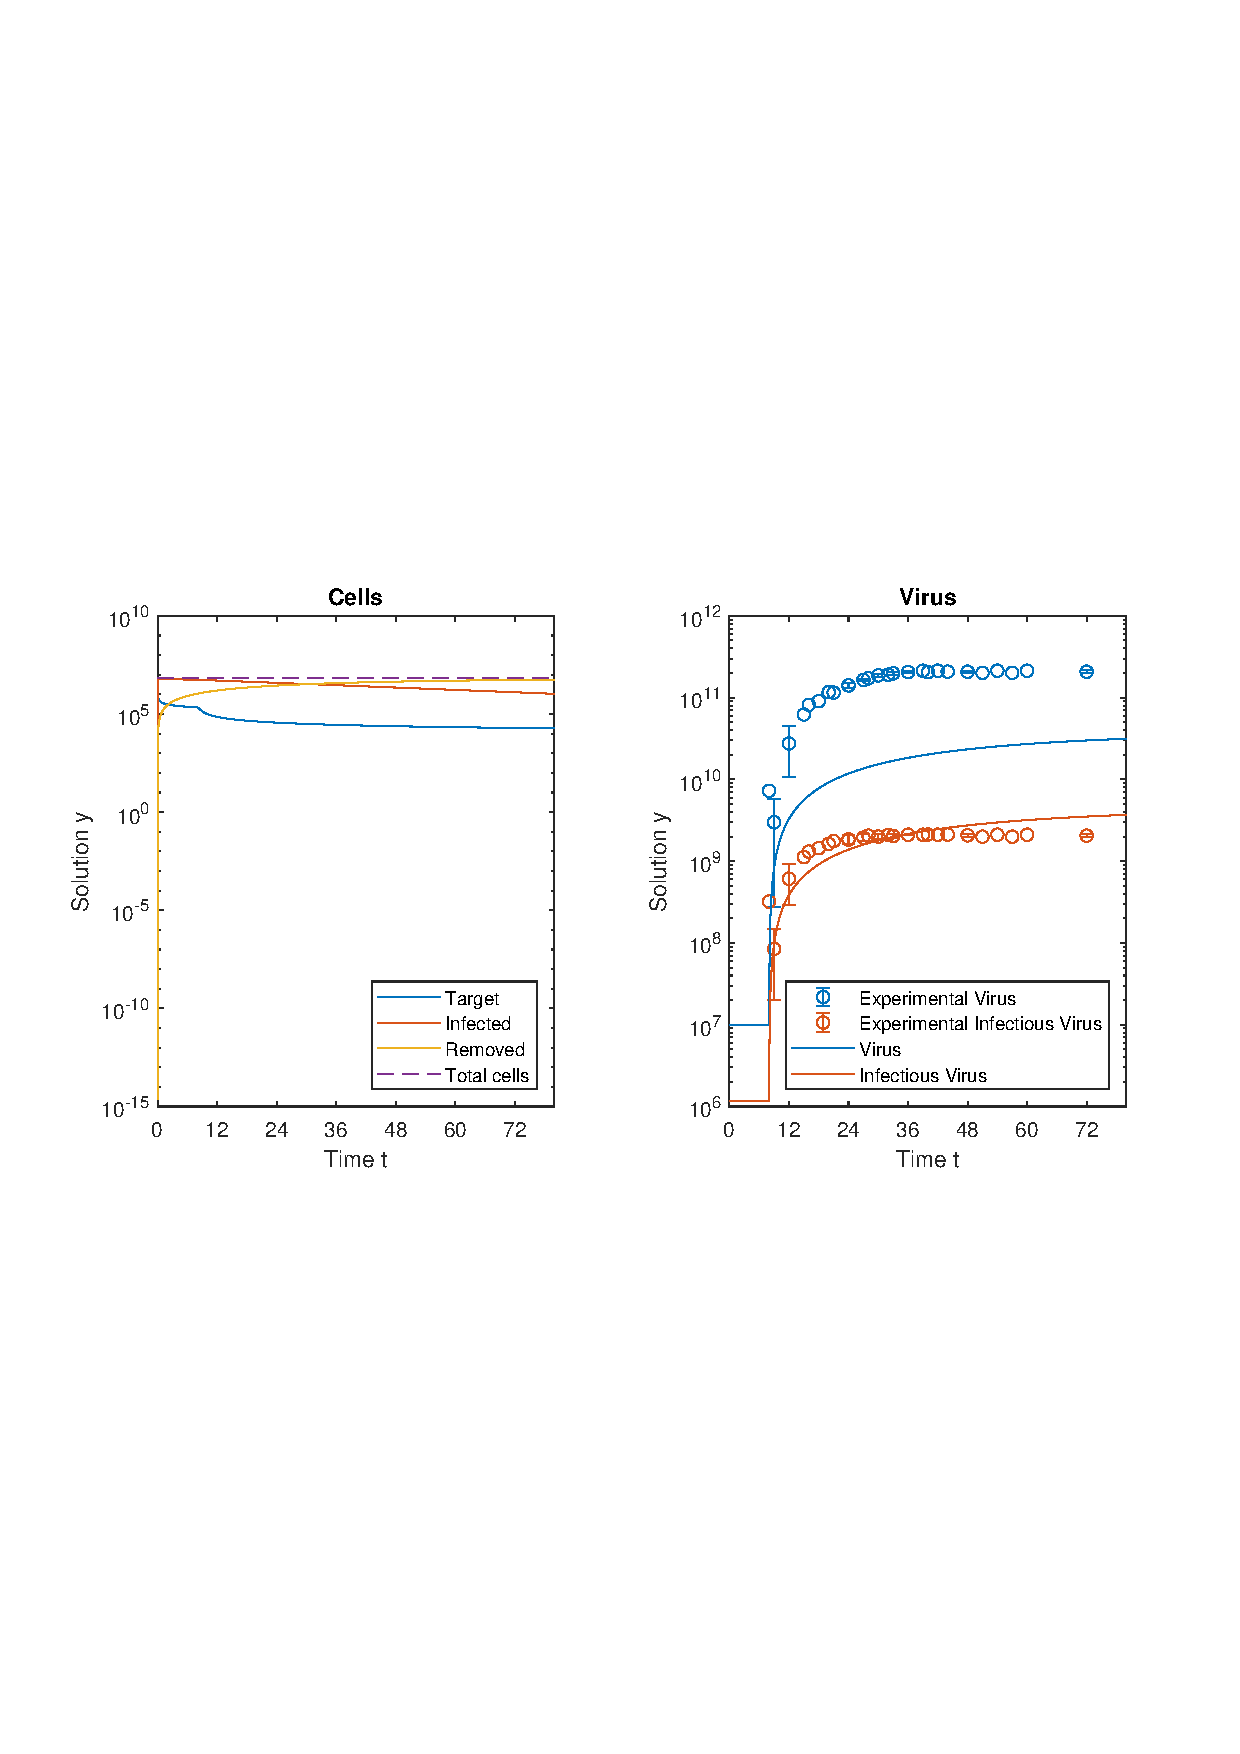
\includegraphics[width=0.6\textwidth, trim={1cm 9.5cm 1cm 9.5cm}, clip]{D_chapters/6_appendix/4_THillIRVViDelay/ModelTHillIRVViDelayDSNSaenz2010FittedMOI3B0.0010133D0.55548P3247.2256C0.0027335TIC1896440.1965TH4.9813iFrac0.11736log.pdf}
\caption[T$_{Hill}$IRVV$_i$, delay $\tau = f(\text{MOI})$ model fit for MOI = 3]%
{T$_{Hill}$IRVV$_i$, delay $\tau = f(\text{MOI})$ model fit for MOI = 3}
\label{figure:THillIRVViDelayMOI3}
\end{center}
\end{figure}

\begin{figure}[H]
\begin{center}
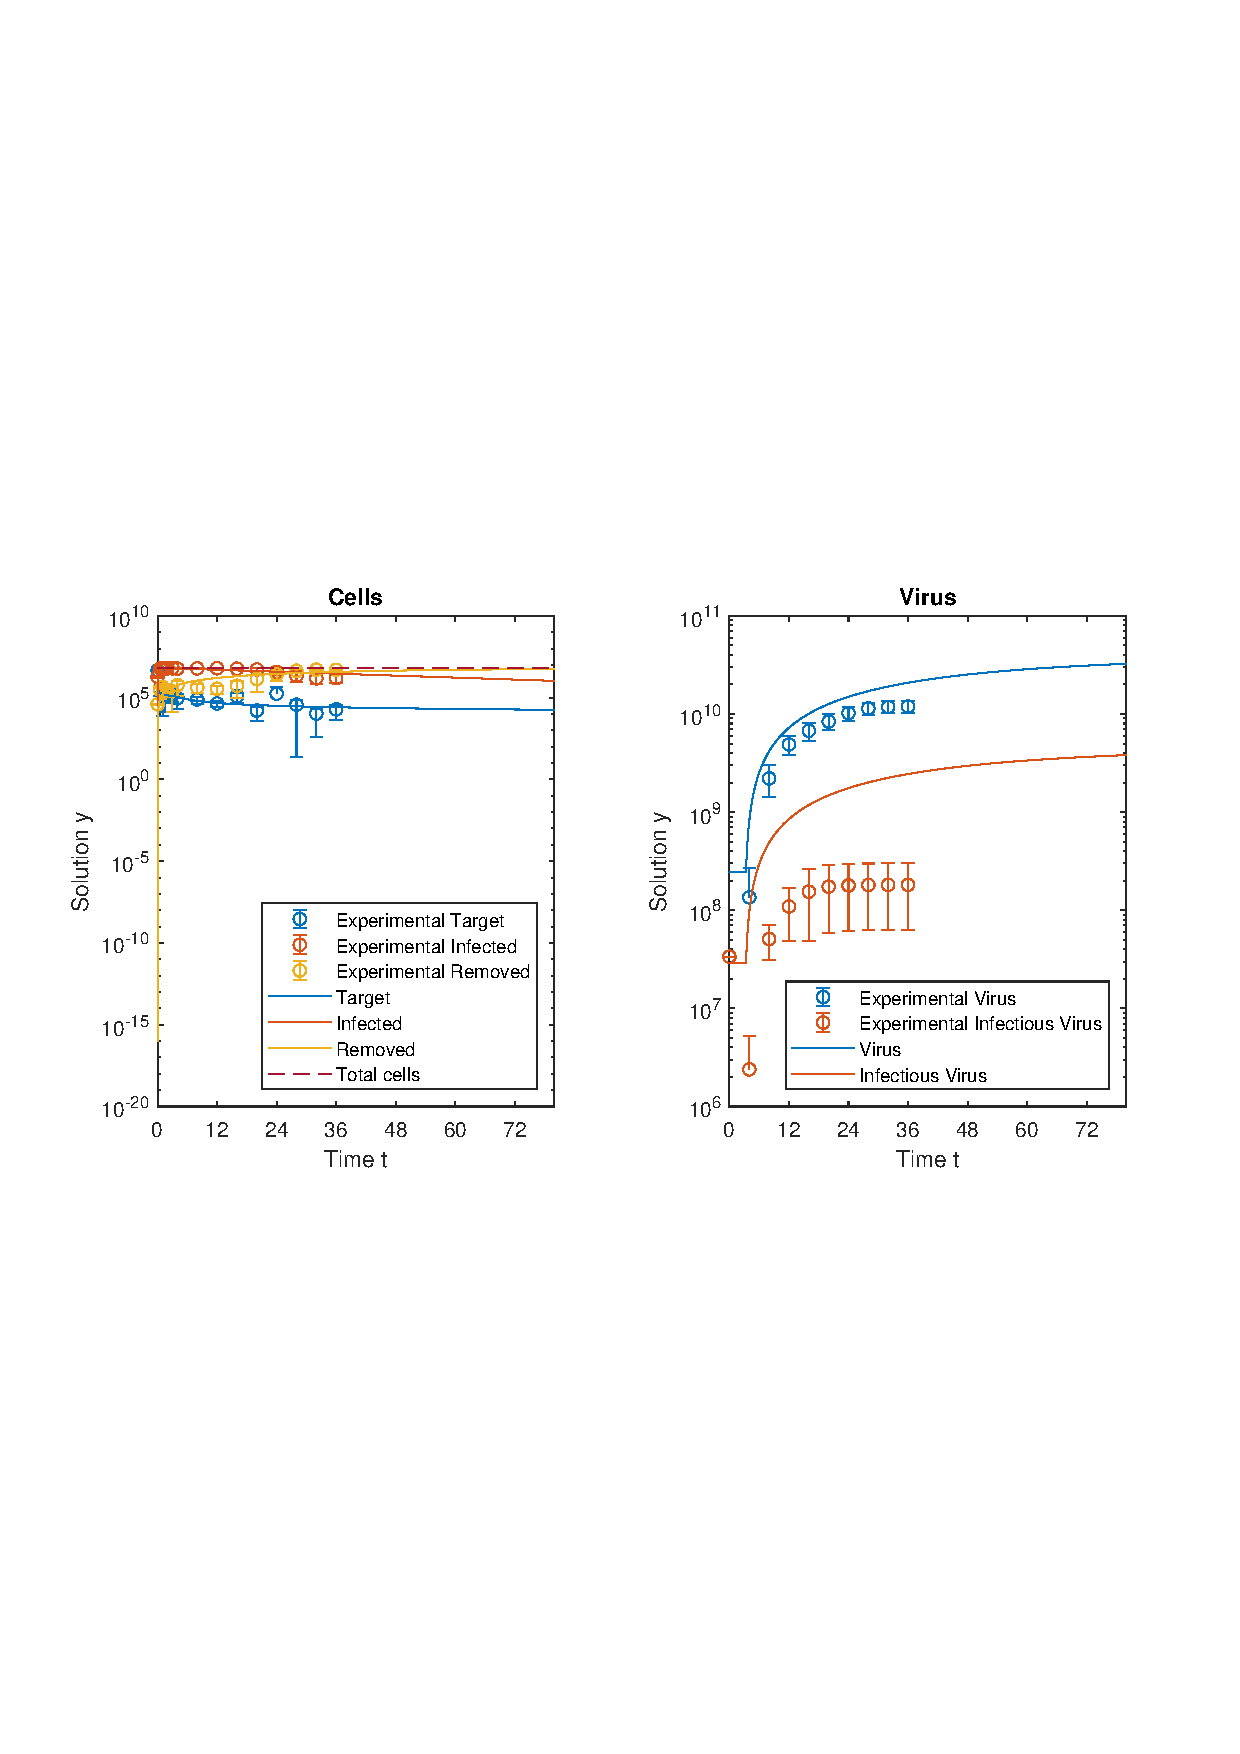
\includegraphics[width=0.6\textwidth, trim={1cm 9.5cm 1cm 9.5cm}, clip]{D_chapters/6_appendix/4_THillIRVViDelay/ModelTHillIRVViDelayDSNSaenz2010FittedMOI73B0.0010133D0.55548P3247.2256C0.0027335TIC1896440.1965TH4.9813iFrac0.11736log.pdf}
\caption[T$_{Hill}$IRVV$_i$, delay $\tau = f(\text{MOI})$ model fit for MOI = 73]%
{T$_{Hill}$IRVV$_i$, delay $\tau = f(\text{MOI})$ model fit for MOI = 73}
\label{figure:THillIRVViDelayMOI73}
\end{center}
\end{figure}

Despite the objective function scores, visual evaluation of the fits (Figures \ref{figure:THillIRVViDelayMOI00001}, \ref{figure:THillIRVViDelayMOI3}, \ref{figure:THillIRVViDelayMOI73}, Appendix \ref{appendix:compartmentalModelFits}, only models which describe target cell population by a fitted Hill equation fits reported) reveals that T$_{Hill}$IRVV$_i$ does not capture the initial delay in the viral production, and all three models struggle to capture the infectious fraction, which in all models is set to be constant (which we know is not the case, as shown on Figure \ref{figure:infectiousFraction}). T$_{Hill}$IRVV$_i$, delay $\tau = f(\text{MOI})$ model predicts an extra viral production bump for low MOI = $10^{-4}$. T$_{Hill}$IRVV$_i$, delay $\tau = const$ suggests one as well, but early in the infection, before the literature reported data points.

\begin{table}[h!]
\centering
\caption[Influenza infection model objective function values for best fits]{Influenza infection model objective function values for best fits}
\label{table:ModelObjFunction}

\begin{tabular}{p{8cm} p{3cm} p{2.5cm}}
\hline 
\textbf{Infection model} & \textbf{Objective function value} & \textbf{Fitted \mbox{parameters}}\\
\hline
chronic TIRVV$_i$ & 2.95 & 6\\
chronic TEIRVV$_i$ & 2.30 & 7\\
\hline
TIRVV$_i$ & 2.96 & 5\\
TEIRVV$_i$ &  3.73 & 6\\
TIRVV$_i$, delay $\tau = f(\text{MOI})$ & 12.82 & 5\\
TIRVV$_i$, delay $\tau = const$ & 6.63 & 6\\
T$_{Hill}$IRVV$_i$ & 0.36 & 7\\
T$_{Hill}$IRVV$_i$, delay $\tau = f(\text{MOI})$ & 0.63 & 7\\
T$_{Hill}$IRVV$_i$, delay $\tau = const$ & 0.25 & 8\\
\hline
\end{tabular}
\end{table}

\newpage

\begin{figure}[H]
\begin{center}
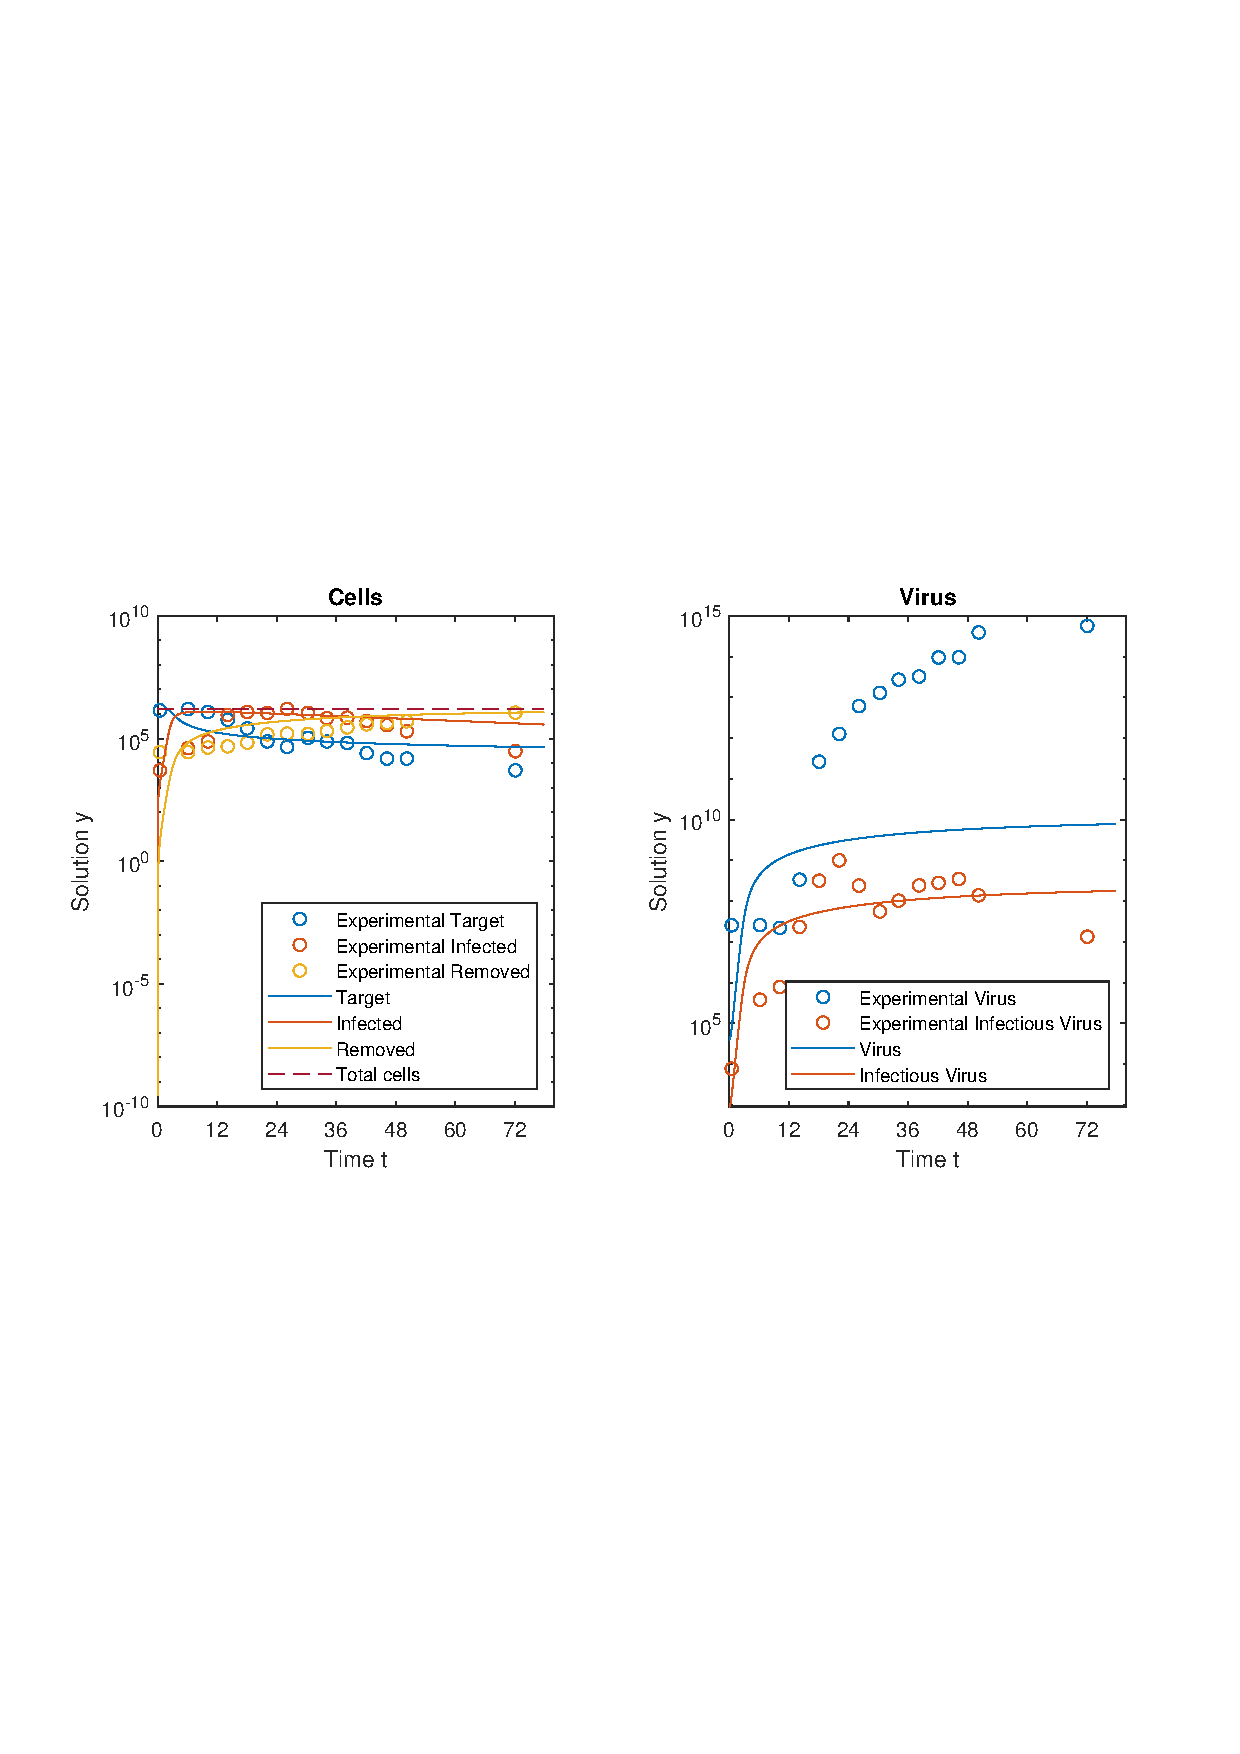
\includegraphics[width=0.65\textwidth, trim={1cm 9.8cm 1cm 9.5cm}, clip]{D_chapters/6_appendix/4_ValidationRKI/InfectionDepletionModelTHillIRVViMOI0.025log.pdf}
\caption[T$_{Hill}$IRVV$_i$ model fit for PR/8/34 H1N1 (RKI)]%
{T$_{Hill}$IRVV$_i$ model fit PR/8/34 H1N1 (RKI)}
\label{figure:THillIRVViValidationRKI}
\end{center}
\end{figure}

\begin{figure}[H]
\begin{center}
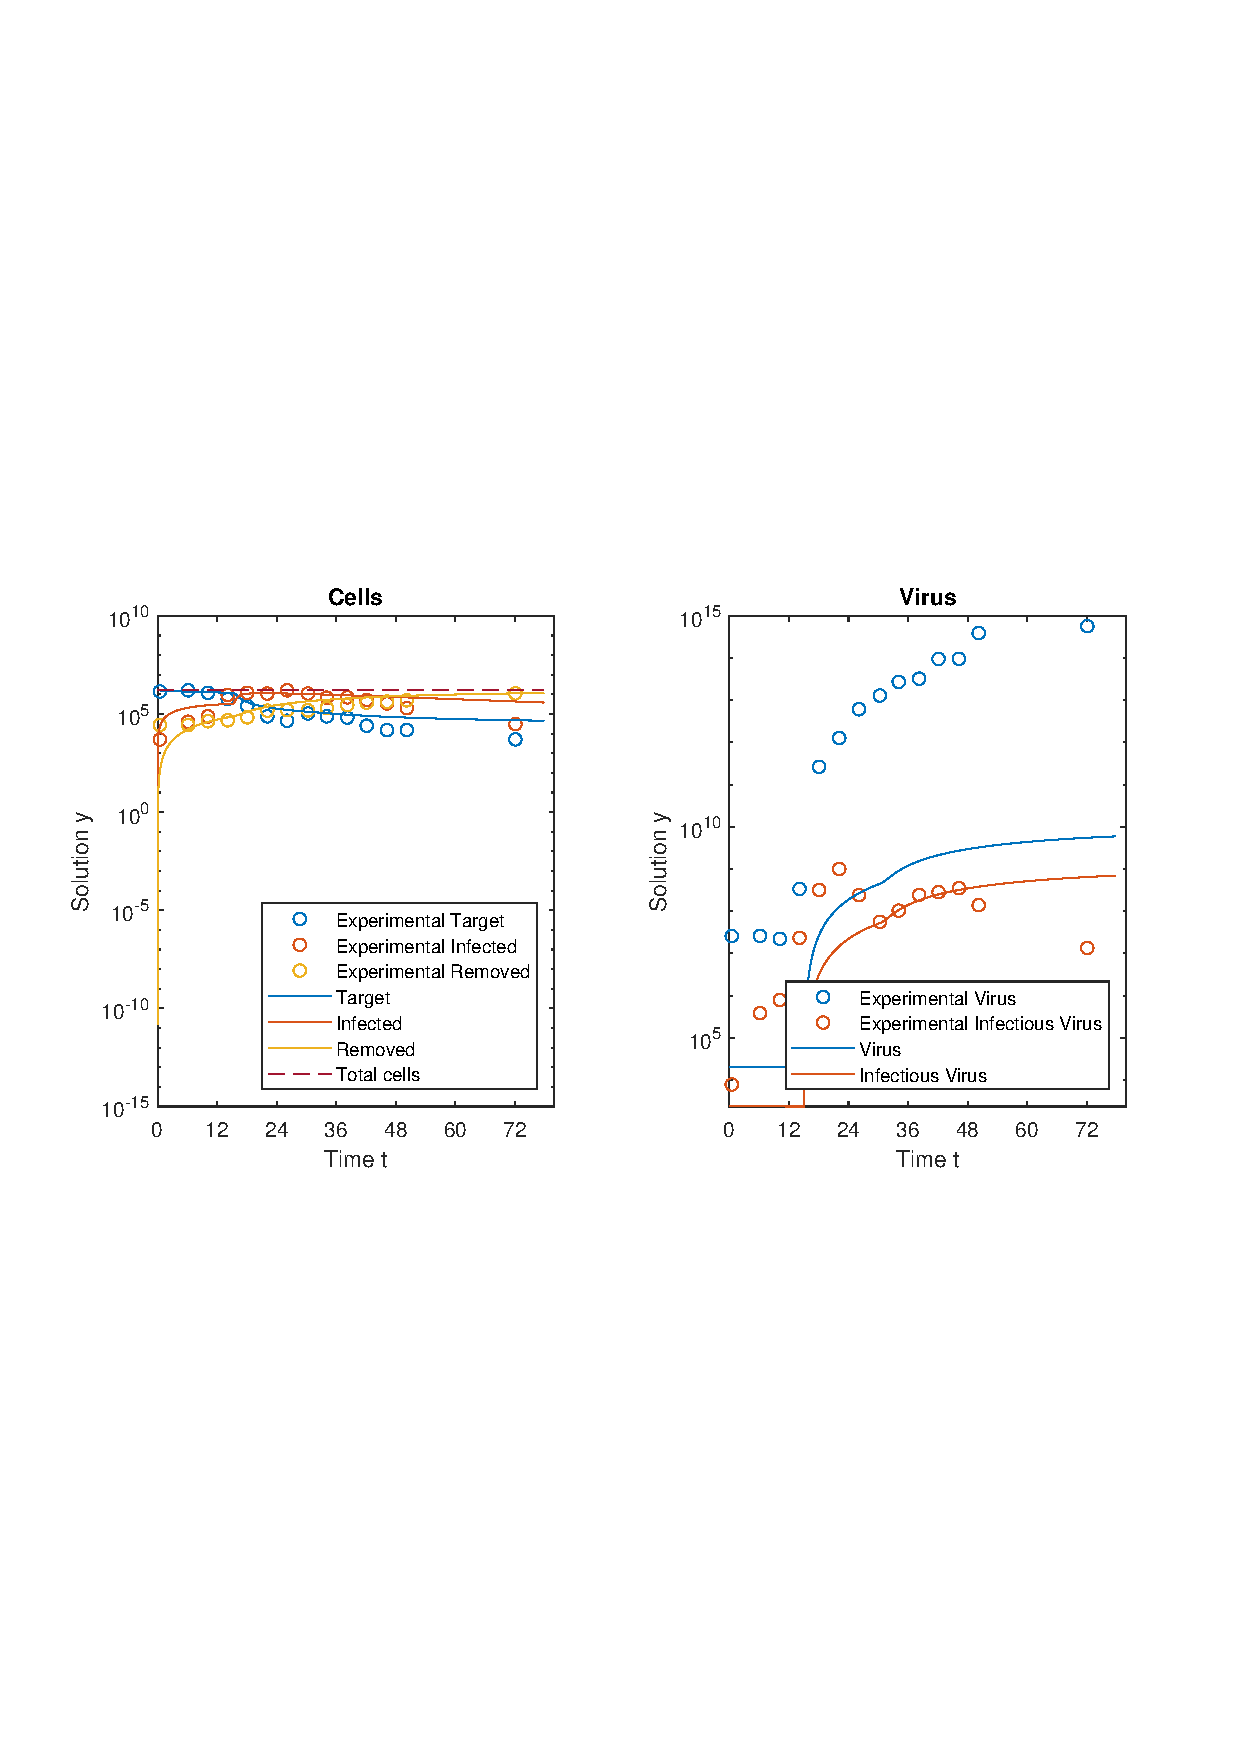
\includegraphics[width=0.65\textwidth, trim={1cm 9.8cm 1cm 9.5cm}, clip]{D_chapters/6_appendix/4_ValidationRKI/InfectionDepletionModelTHillIRVViDelayMOI0.025log.pdf}
\caption[T$_{Hill}$IRVV$_i$, delay $\tau = f(\text{MOI})$ model fit forPR/8/34 H1N1 (RKI)]%
{T$_{Hill}$IRVV$_i$, delay $\tau = f(\text{MOI})$ model fit for PR/8/34 H1N1 (RKI)}
\label{figure:THillIRVViDelayValidationRKI}
\end{center}
\end{figure}

\begin{figure}[H]
\begin{center}
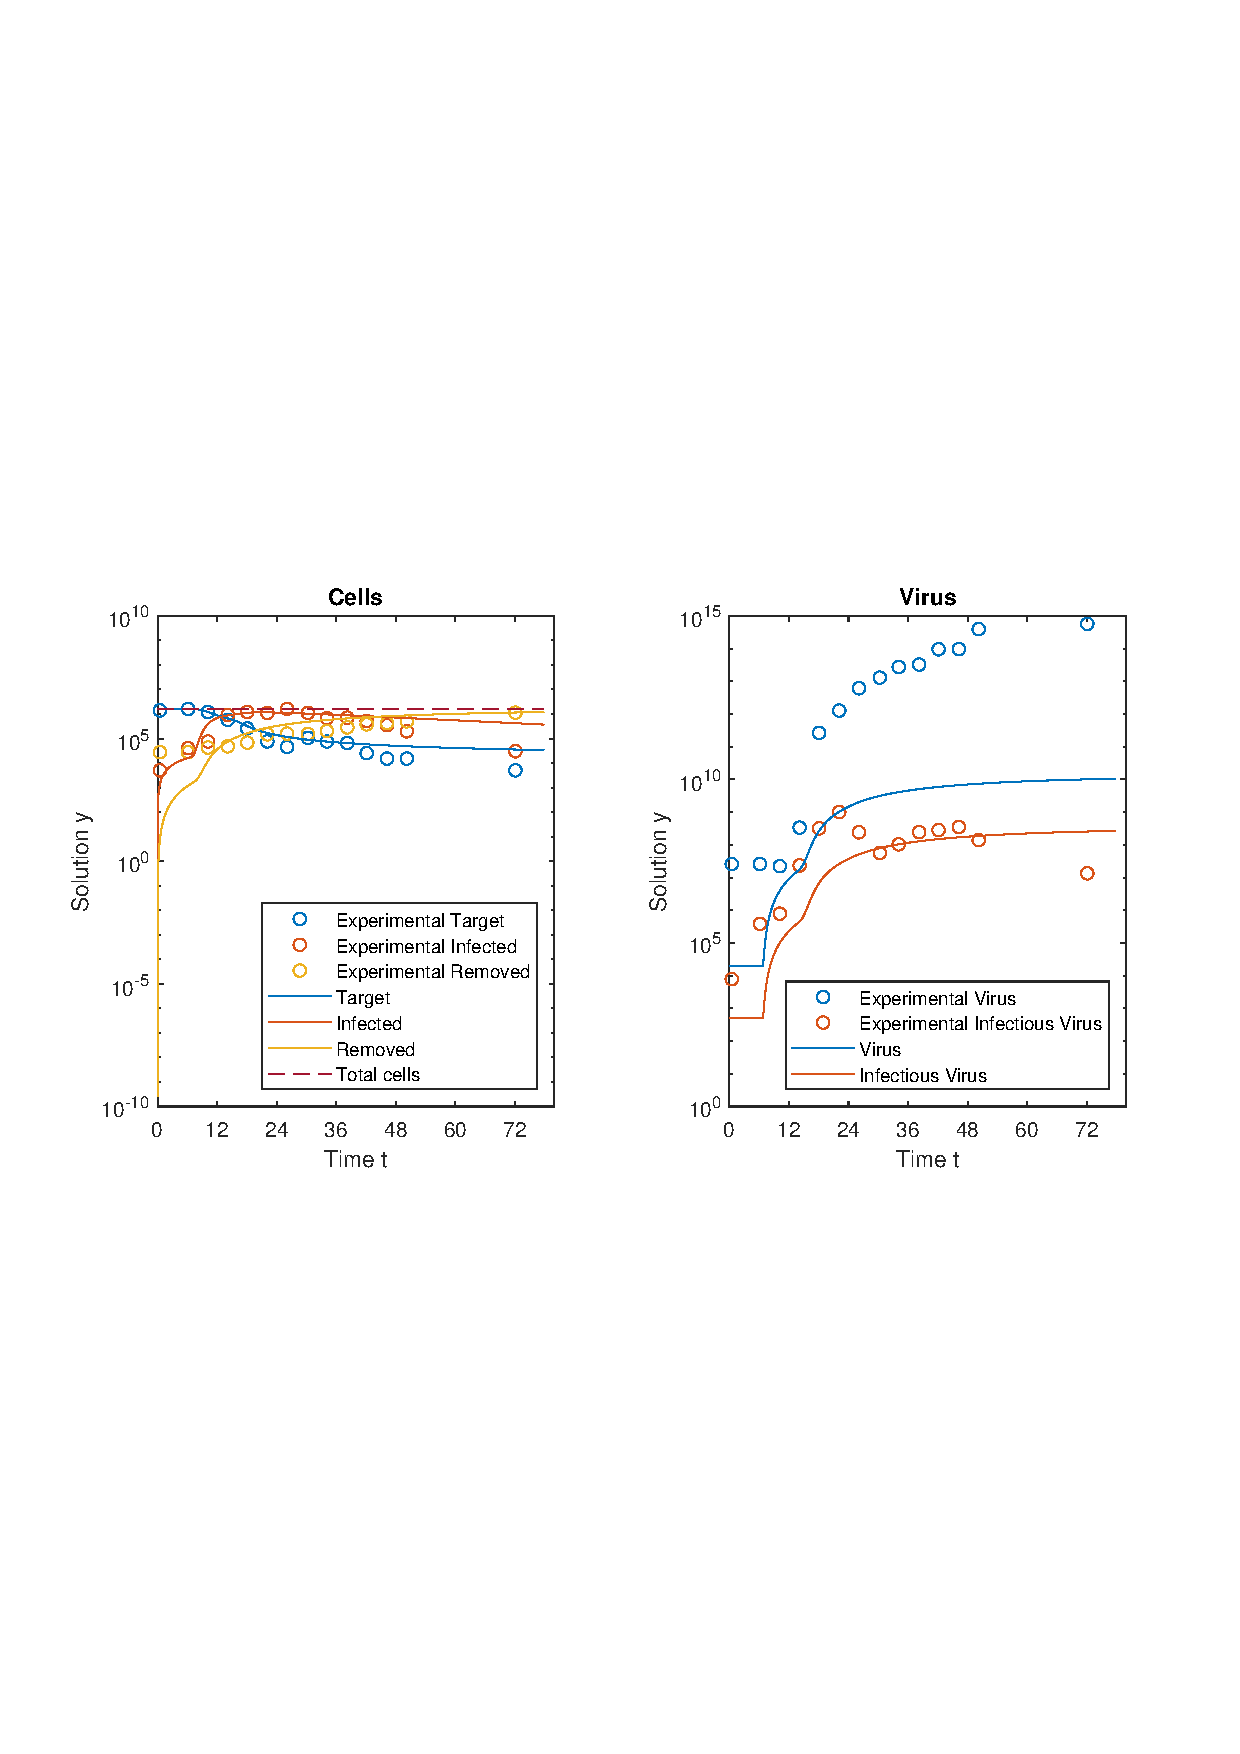
\includegraphics[width=0.65\textwidth, trim={1cm 9.8cm 1cm 9.5cm}, clip]{D_chapters/6_appendix/4_ValidationRKI/InfectionDepletionModelTHillIRVViDelayFitTauMOI0.025log.pdf}
\caption[T$_{Hill}$IRVV$_i$, delay $\tau = const$ model fit for PR/8/34 H1N1 (RKI)]%
{T$_{Hill}$IRVV$_i$, delay $\tau = const$ model fit for PR/8/34 H1N1 (RKI)}
\label{figure:THillIRVViDelayFitTauValidationRKI}
\end{center}
\end{figure}

To evaluate the practical usability of these fits, we used them to run the simulations with initial conditions corresponding to the ones reported in \cite{schulze2009infection}, and visually compared the resulting trajectories with digitized data from \cite{schulze2009infection}. For all the viral strains our best fit candidates again performed the best (Figures \ref{figure:THillIRVViValidationRKI}, \ref{figure:THillIRVViDelayValidationRKI}, \ref{figure:THillIRVViDelayFitTauValidationRKI}, Appendix \ref{appendix:compartmentalModelFitValidation}). However, all three models struggled significantly to capture the infectious fraction. As previously discussed, this discrepancy may be explained by the infectious fraction in \cite{schulze2009infection} being significantly reduced compared to our fitting data \cite{rudiger2019multiscale}. Interestingly, for PR/8/34H1N1 (RKI) and WSN/67/2005 HGR H3N2 strains the infectious virions trajectory was simulated reasonably well by the models, unlike for PR/8/34H1N1 (NIBSC), which had the worst infectious fraction out of all the strains reported in \cite{schulze2009infection}.

Out of all the simulated models T$_{Hill}$IRVV$_i$, delay $\tau = const$ and T$_{Hill}$IRVV$_i$, delay $\tau = f(\text{MOI})$ seem to perform the best, in terms of capturing both cellular behavior and overall shape of the viral production. Unfortunately, we cannot say that modelling delay $\tau = f(\text{MOI})$ as a function of MOI offers any significant advantage over $\tau = const$, but it is worth noting that $\tau = const$ requires fitting $\tau$ as an additional parameter of the infection model, where $\tau = f(\text{MOI})$ relies on a pre-computed expression.

\subsection{DARPin-F10 drug-like activity}

To model the drug-like activity of DARPin-F10, we modified our fitted infection models T$_{Hill}$IRVV$_i$, delay $\tau = const$ and T$_{Hill}$IRVV$_i$, delay $\tau = f(\text{MOI})$ to include DARPin-F10. Ultimately, both model variants have produced qualitatively similar results, so here we only present the simulation results for T$_{Hill}$IRVV$_i$, delay $\tau = f(\text{MOI})$.

We examined two possible cases: one where DARPin-F10 behaves similarly to amantadine drug, reducing the infection rate $\beta$, and another, where it behaves similarly to neuraminidase inhibitors, reducing the virion production $p$.

To model DARPin-F10 influence on the infection we used parametrised dose response curves (Table \ref{table:DARPinFittingCoefficients}) obtained from modified HDAC6 complex formation models "Asymmetric DARPin" and "Symmetric DARPin" to compute the drug effect, under assumption that the DARPin-F10 concentration stays constant throughout simulation. Since in the limit where DARPin-F10 = 0 our predictions for dose response would be the same as the WT conditions, for simplicity we assumed that $\epsilon_{max} - \epsilon_{min} = 1$. Both "Asymmetric DARPin" and "Symmetric DARPin"  sets of parameters produced qualitatively similar results, so here we only present the results for "Asymmetric DARPin".

Surprisingly, an amantadine-like model (Figure \ref{figure:amantadineLikeF210}, Appendix \ref{appendix:amantadineDarpin}) only led to a moderate decrease in viral production. In this model DARPin-F10 reduces infection rate $\beta$, leading to slower target cell depletion (Figure \ref{figure:amantadineLikeF210}, orange line), to a slower increase in the number of infected cells (Figure \ref{figure:amantadineLikeF210}, yellow line), and to less steep virus production (Figure \ref{figure:amantadineLikeF210}, blue line). This model captures the overall smoother shape of the DARPin-F10 inhibited viral growth at the start of the infection (Figure \ref{figure:amantadineLikeF210}, $\le 36$ hours), but the simulated virus production does not quite reach experimentally observed reduction even at high concentration of DARPin-F10 (Figure \ref{figure:amantadineLikeF210} $[F]_{effective}$ = 210.24 = 7.3 $\mu$M.

\begin{figure}
\begin{center}
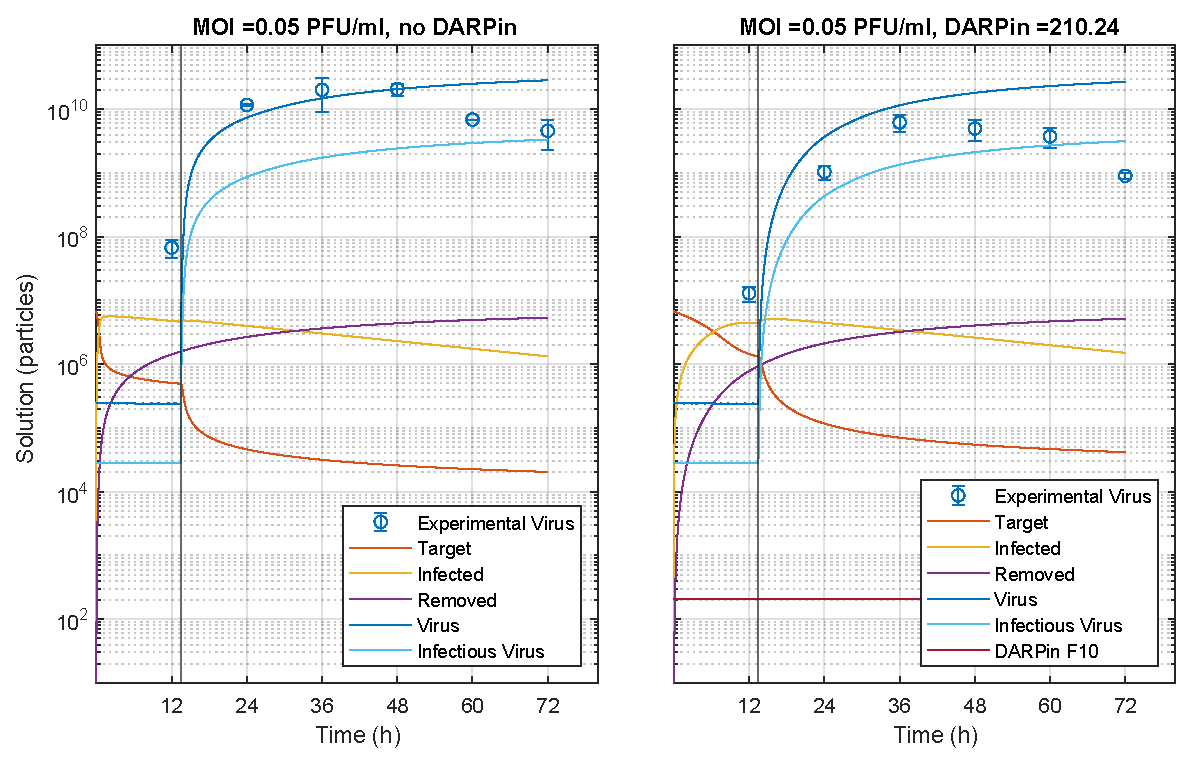
\includegraphics[width=0.8\textwidth, trim={0cm 0cm 0cm 0cm}, clip]{D_chapters/3_DARPinModels/2_DARPinInfection/comparisonModelTHillIRVViDelayMOI0.072135DARPin210.236AsymmetricDarpinMyosinInhibitor.pdf}
\caption[Amantadine-like DARPin-F10 for MOI = 0.05 PFU/ml and $F_{effective}$ = 210.24]{Amantadine-like DARPin-F10 influence on the influenza infection for MOI = 0.05 PFU/ml and relative DARPin-F10 $[F]_{effective}$ = 210.24, calculated based on viral growth curves at MOI = 10 PFU/ml. Experimental data is normalized to  the simulated virus production value at 48h for no DARPin case.}
\label{figure:amantadineLikeF210}
\end{center}
\end{figure}

Neuraminidase inhibitor-like models (Figures \ref{figure:neuraminidaseInhibitorLikeF62}, Appendix \ref{appendix:neuraminidaseInhibitorDarpin}) were able to capture the reduction in viral production far more successfully, particularly for $[F]_{effective}$ = 62.69 = 2.2 $\mu$M, determined from viral growth curves at MOI = 0.05 PFU/ml (Figure \ref{figure:neuraminidaseInhibitorLikeF62}). In this model DARPin-F10 reduces production rate $p$, directly decreasing the numbers of total (Figure \ref{figure:neuraminidaseInhibitorLikeF62}, blue line) and infectious (Figure \ref{figure:neuraminidaseInhibitorLikeF62}, light blue line) virus in the system. This may indicate that inhibition of HDAC6-Ub binding during HDAC6-mediated uncoating leads to disruption of HDAC6-assisted viral particle assembly.

\begin{figure}
\begin{center}
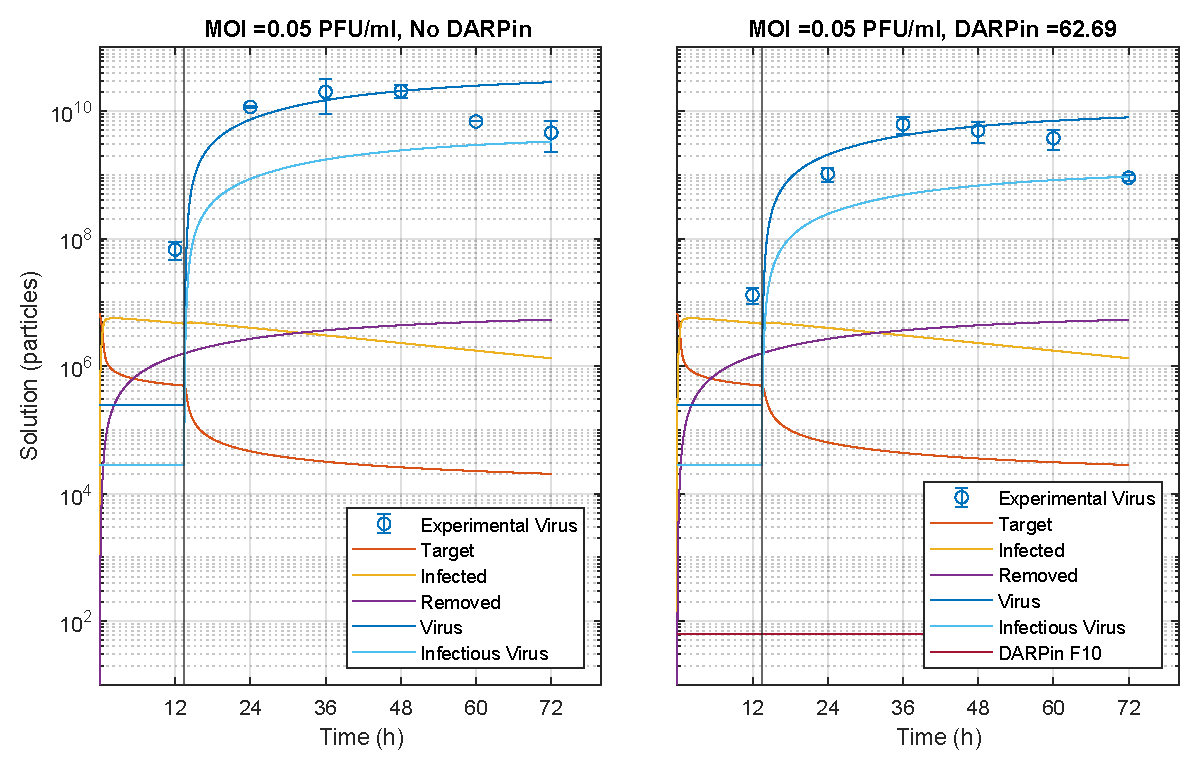
\includegraphics[width=0.8\textwidth, trim={0cm 0cm 0cm 0cm}, clip]{D_chapters/3_DARPinModels/2_DARPinProduction/comparisonModelTHillIRVViDelayMOI0.072135DARPin62.6898AsymmetricDarpinMyosinInhibitor.pdf}
\caption[Neuraminidase inhibitor-like DARPin-F10 for MOI = 0.05 PFU/ml and $F_{effective}$ = 62.69]{Neuraminidase inhibitor-like DARPin-F10 influence on the influenza infection for MOI = 0.05 PFU/ml and relative DARPin-F10 $[F]_{effective}$ = 62.69, calculated based on viral growth curves at MOI = 0.05 PFU/ml. Experimental data is normalized to the simulated virus production value at 48h for no DARPin case.}
\label{figure:neuraminidaseInhibitorLikeF62}
\end{center}
\end{figure}

\section{Discussion}

When dose-response models are discussed, usually they are based on experimentally measured effects in, for example, cell culture. As far as we're aware, the use of another biochemical-biophysical model for such purpose is a conceptual novelty. Admittedly, the underlying biochemical model relies on simple bimolecular reactions equations, which might not necessarily be the case for actual proteins involved. However, the overall approach is not at all limited to bimolecular reactions, and can be extended to include any amount of interaction detail, given reasonable estimates of concentrations and reaction rates.

Our estimates of DARPin-F10 effective concentrations rely on experimental observations of DARPin-F10 efficacy. Under the assumption that DARPin-F10 inhibits HDAC6-mediated influenza uncoating, the uncoating experiment (Figure \ref{figure:darpinUncoatingExperimental}) should provide the best estimate. However, in this uncoating experiment a much higher viral titer with MOI = 30 PFU/ml has been used (in comparison, \cite{banerjee2014influenza} report MOI = 1 in MEF experiments), possibly leading to lower estimates of DARPin-F10 efficiency. Further, our model predictions rely on knowledge of reaction rates. While experimental data provides an estimate of dissociation rate $K_{HF}$ between DARPin-F10 and HDAC6, we use an average rate of bimolecular reaction \cite{bionumbersbimolrate} as an estimate for on-rate $k_{HF}$. Given that it controls how quickly the binding happens, it is possible we underestimate the actual amount of HDAC6-bound DARPin-F1. This may lead to a higher estimate for effective concentrations than what's actually required for uncoating inhibition.

Non-structured kinetic models are quite attractive in their basic idea - by simply determining the initial amounts of cells and the virus we can predict the trajectories of the viral infection. However, quite often their use is limited to simply calculating reproductive number $R_0$. One reason for such limited use is implicit assumptions coming from fitted parameters. This aspect is obvious when we examine in the variability of model parameters between different publications \cite{smith2011influenza}. Another difficulty is differences in preparation protocols, as we can clearly see in infectious fraction differences between \cite{rudiger2019multiscale} and \cite{schulze2009infection} (Figure \ref{figure:infectiousFraction}). Finally, the use of non-structured model makes it difficult to make any mechanistic predictions which aren't already apparent from the underlying data.

Here we tried to circumvent this issue by combining those non-structured kinetic models with simple data-driven models, which aim to untangle the implicit relationships between initial conditions and parameters (Figures \ref{figure:delayMoiValidation}, \ref{figure:infectiousFraction}). Unfortunately, infectious fraction analysis was complicated by strong differences between the two used datasets, and use of just single dataset with only 3 datapoints is hardly justified for this purpose. Nevertheless, we believe that this approach warrants future attempts.

Our suggested relationship between $\tau_{delay}$ and MOI is  only based on 5 datapoints. Despite this sparsity of data, it seems to capture the results in human and cell culture reasonably well (Figure \ref{table:delayTauValidation}). However, within the framework of kinetic models we weren't able to conclusively prove an advantage of using it over a simple T$_Hill$IRVV$_i$, $\tau_{delay} = const$ fit. The two models seem to describe the fitting and validation data similarly well, and the only improvement our T$_Hill$IRVV$_i$, $\tau_{delay} = f(MOI)$ offers is a reduction in number of fitted kinetic model parameters by 1. Here we assume the delay value $\tau_{delay}$ can be directly observed from the viral growth trajectories. Judging from the simulation results of $\tau_{delay} = const$ that might not necessarily be the case, and it's entirely possible that MOI rather affects, for example, infection rate $\beta$ (since higher number of viral particles would increase the probability of target cells getting infected). 

Given these difficulties with implementing a basic robust kinetic infection model, our conclusions about the role of DARPin-F10 have to be taken with a grain of salt. Specifically, our measure of DARPin-F10 efficacy on viral growth curves is based on the total produced virus trajectories, however, both fitting and validation of kinetic models highlighted that even our best kinetic models struggle to fully capture viral production. Ultimately, it may be useful to not only focus the experiments on total viral production, but also include cellular trajectories and infectious viral production, since uncoating inhibition may increase the production of DIPs reducing observed infectious fraction.

Despite these difficulties, based on our simple kinetic models of DARPin-F10 effect we can confirm the observation \cite{heldt2013multiscale} that drug interventions targeting viral production are more efficient at achieving reduction in viral titer than interventions targeting primarily targeting viral entry. Additionally, that raises a question of whether uncoating inhibitions counts as rather first or the second, or neither, requiring higher level of precision in kinetic model implementation.

\section{Methods}

\subsection{Modified HDAC6 complex formation models}

We created two new HDAC6 complex formation models including DARPin-F10 as a competitor against Ub for HDAC6-Znf binding. These models are based on previously described "Symmetric" and "Asymmetric" model variants. Detailed model equations are described in Appendix \ref{appendix:DARPinModelsEquations}.

To compare original and modified HDAC6 complex formation models we uniformly sampled the rates and concentrations, as was previously described (Chapter \ref{ch:ReactionModels}) for original "Symmetric" and "Asymmetric" (Figure \ref{figure:darpinDensities}). We used two different predetermined concentrations of DARPin-F10. Based on \cite{guillard2017structural}, who report half maximal inhibitory concentration ($IC_{50}$) for DARPin-K27 and DARPin-K55 in range between 2.4 to 67 nM in their experiments, we chose $34.7$ nM as an estimate for an active concentration of DARPin-F10, and  $34.7 \cdot 10^{-6}$ nM as a negligible DARPin concentration case. For on-rate of HDAC6 and DARPin-F10 binding $k_{HF}$ we chose $10^{6} \frac{1}{s\cdot M}$ - average rate of bimolecular reaction \cite{bionumbersbimolrate}. For dissociation constant $K_{HF}$ we used $90$ nM \cite{DarpinData}.

To determine the impact of DARPin-F10 concentration on uncoating we fixed all the other concentrations and rates, sampled widely in the range of $\pm$ 5 orders of magnitude around of chosen literature value. We fitted both trajectories as a Hill equation using log-logistic function \texttt{LL.4()} from R package \texttt{drc}:

\begin{equation}
\epsilon=\frac{\epsilon_{max} - \epsilon_{min}}{1 + \big(\frac{[F]}{EC_{50}}\big)^n}
\end{equation}

where $\epsilon_{max}$ and $\epsilon_{min}$ are maximal and minimal drug efficacy, respectively, $[F]$ is DARPin F10 concentration, $EC_{50}$ is half maximal effective concentration of DARPin F10, and $n$ is a Hill coefficient.

To compute DARPin concentration $[F]_{effective}$ corresponding to experimentally observed uncoating (Figure \ref{figure:darpinUncoatingExperimental}) and viral growth (Figure \ref{figure:darpinGrowthExperimental}) reduction, we used the following formula:

\begin{equation}
[F]_{effective} = \exp\big( \frac{1}{n}\cdot\log( \frac{\epsilon_{max}-\epsilon_{min}}{\epsilon_{max}\cdot\omega - \epsilon_{min}} - 1 ) +\log(EC_{50}) \big)
\label{eq:darpinEffectiveConcentration}
\end{equation}

where $\omega = \text{avg}(\frac{x_{DARPin}(t)}{x_{WT}(t)})$ is an observed fraction of efficiency for observations $x$ at time points $t$.

Using the data \cite{DarpinData} provided by our collaborators we determined that for uncoating experiment (Figure \ref{figure:darpinUncoatingExperimental}) at MOI = 30 PFU/ml corresponding efficiency of uncoating, compared to the wild type (WT) has been at approximately $\omega$ = 73\%. By comparing the averages of viral growth in presence of DARPin-F10 (Figure \ref{figure:darpinGrowthExperimental}) at MOI = 0.05 and 10 PFU/ml for data points >12 and $\ge$8 hours respectively, we determined that DARPin-F10 presence reduced viral growth respectively to $\omega$ = 31\% and $\omega$ = 11\% of WT. Using these values and Equation \ref{eq:darpinEffectiveConcentration} we can obtain estimates for DARPin-F10 effective concentration (Table \ref{table:DARPinFittingCoefficients}).

\begin{table}[h!]
\centering
\caption[Fitted Hill equation parameters and effective DARPin-F10 concentrations]{Fitted Hill equation parameters and effective DARPin-F10 concentrations based on sampling HDAC6 complex formation models.}
\label{table:DARPinFittingCoefficients}

\begin{tabular}{p{5cm} p{3cm} p{3cm}}
\hline 
\textbf{Parameter} & \textbf{Asymmetric DARPin} & \textbf{Symmetric DARPin}\\
\hline
$n$ &                 1.37&    1.48\\
$\epsilon_{min}$ &    0.03&    -0.01\\
$\epsilon_{max}$ &    0.78&    0.65\\
$EC_{50}$, relative &          31.54&    49.85\\
$EC_{50}$, $\mu$M &          1.1&    1.7\\
\hline
\multicolumn{3}{l}{$\omega$ = 73\%, uncoating assay}\\
$[F]_{effective}$, relative & 15.82 & 25.08\\
$[F]_{effective}$, $\mu$M & 0.5 & 0.9\\
\hline
\multicolumn{3}{l}{$\omega$ = 31\%, viral growth curves, MOI=0.05 PFU/ml}\\
$[F]_{effective}$, relative & 62.69 & 83.52\\
$[F]_{effective}$, $\mu$M & 2.2 & 2.9\\
\hline
\multicolumn{3}{l}{$\omega$ = 11\%, viral growth curves, MOI=10 PFU/ml}\\
$[F]_{effective}$, relative & 210.24 & 194.85\\
$[F]_{effective}$, $\mu$M & 7.3 & 6.8\\
\hline
\end{tabular}
\end{table}

\subsection{Functional analysis of literature available data}

We used the raw data for influenza infection for three different MOI = $10^-4$, $3$, $73$ reported in the supplement of \cite{rudiger2019multiscale}, to plot influenza infection total virus growth trajectory and fit it using asymptotic regression function \texttt{AR.3()} from R package \texttt{drc}:

\begin{equation}
f(x) = c + (d-c)\big(1-\exp(-\frac{t}{e})\big)
\label{eq:ar3function}
\end{equation}

The parameter $c$ is the lower limit at $t=0$, the parameter $d$ is the upper limit, and the parameter $e>0$ is determining the steepness of the increase with $t$.

Analogously, we fitted the WT DARPin viral growth curves provided to us by our collaborators \cite{DarpinData} (Figure \ref{figure:totalVirusFits}).

\begin{figure}
\begin{center}
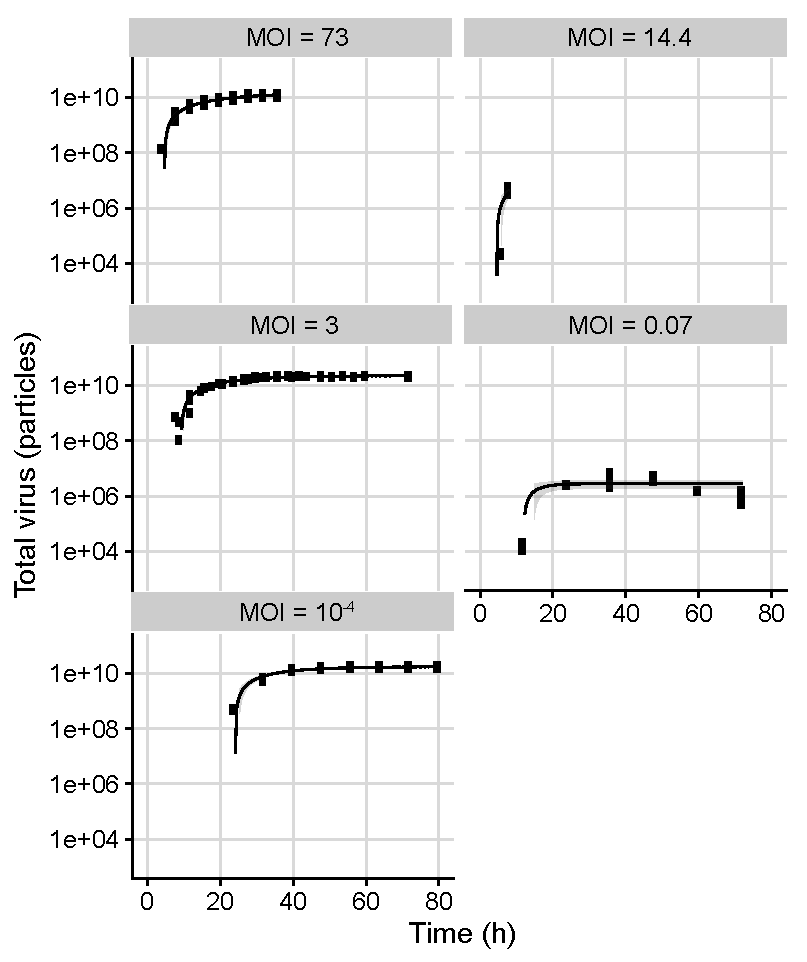
\includegraphics[width=0.8\textwidth, trim={0cm 0cm 0cm 0cm}, clip]{D_chapters/3_DARPinModels/fittingTotalVirus.pdf}
\caption[Total virus fits]{Total virus fits using \cite{rudiger2019multiscale, DarpinData} data.}
\label{figure:totalVirusFits}
\end{center}
\end{figure}

Our collaborators measure MOI in PFU/ml, while \cite{rudiger2019multiscale} used 50\% tissue culture infectious dose (TCID$_50$) assay to measure it. To convert PFU/ml units into approximate TCID$_50$ we used Poisson distribution:

\begin{equation}
P = \exp(-MOI_{mean})
\end{equation}

where $MOI_{mean}$ is a mean number of infectious units per volume is expressed in PFU/ml units. For any titer expressed in TCID$_50$ P = 0.5, giving us $MOI_{mean} = -\log(0.5)$. Under assumption that the protocol changes do not affect viral production, we convert PFU/ml to TCID$_50$ we divide corresponding MOI measurements by $MOI_{mean}$, giving us MOI = 10 PFU/ml = 14.4, and MOI = 0.05 PFU/ml = 0.07.

To calculate the delay time for each value of MOI we used Equation \ref{eq:ar3function} and compute the $\tau_{delay}$ value corresponding to $f(x) = 0$:

\begin{equation}
\tau_{delay} = -e\log(1+\frac{c}{d-c})
\end{equation}

We then fitted $\tau_{delay}$ as a function of MOI (Equation \ref{eq:delayMOI}) using R function \texttt{lm} from package \texttt{stats}.

To validate this equation, we digitized viral production curves reported in \cite{baccam2006kinetics, handel2007neuraminidase, handel2010towards, smith2011effect, miao2010quantifying, mohler2005mathematical} using WebPlotDigitizer \cite{Rohatgi2020} tool, fitted and computed corresponding $\tau_{delay}$ values, and used or calculated used MOI based on the number of cells and virus used in the experiments (Table \ref{table:delayTauValidation}, Figure \ref{eq:delayMOI}).

\begin{table}[h!]
\centering
\caption[$\tau_{delay} = f(MOI)$ validation]{$\tau_{delay} = f(MOI)$ validation based on digitized literature data.}
\label{table:delayTauValidation}

\begin{tabular}{p{2cm} p{2cm} p{2cm} p{2cm} p{4cm}}
\hline 
\textbf{Data} & \textbf{MOI} & \textbf{$\tau_{delay}$ (h)} &  \textbf{Species} & \textbf{Strain}\\
\hline
\cite{baccam2006kinetics} & $4\cdot 10^{-5}$ & 27.4 & human & A/Hong Kong/123/77 (H1N1)\\
\cite{handel2007neuraminidase} & $1\cdot 10^{-4}$ & 24.1 & human & A/Texas/91 (H1N1)\\
\hline
\cite{handel2010towards} & $1.7$ & 32.0 & mouse & A/Puerto Rico/8/34 (H1N1)\\
\cite{smith2011effect} & $1\cdot 10^{-5}$ & 13.5 & mouse & A/Puerto Rico/8/34 (H1N1) with PB1-F2(1918)\\
\cite{smith2011effect} & $1\cdot 10^{-5}$ & 19.2 & mouse & A/Puerto Rico/8/34 (H1N1)\\
\cite{miao2010quantifying} & $5\cdot 10^{-3}$ & 7.6 & mouse & A/Hong  Kong/X31 (H3N2)\\
\hline
\cite{schulze2009infection} & 0.025 & 15.0 & MDCK & A/Puerto Rico/8/34 (H1N1) NIBSC\\
\cite{schulze2009infection} & 0.025 & 17.5 & MDCK & A/Puerto Rico/8/34 (H1N1) RKI\\
\cite{schulze2009infection} & 0.002 & 16.5 & MDCK & WSN/67/2005 (H3N2)\\
\cite{mohler2005mathematical} & 0.025 & 14.2 & MDCK & A/equine/ Newmarket /1/93 (H3N8)\\
\hline
\end{tabular}
\end{table}

To analyze the infectious fraction change over time we plotted the data reported in \cite{rudiger2019multiscale, schulze2009infection}, and fitted it as a parallel slope model using using R function \texttt{lm} from package \texttt{stats}:

\begin{equation}
\log(\text{Infectious fraction}) = a + b \cdot t
\end{equation}

where $t$ is time, $b$ is a slope coefficient, and $a$ is an intercept, conditional on MOI \cite{rudiger2019multiscale} or viral strain \cite{schulze2009infection} (Table \ref{table:linearFitsInfectiousFraction}).

\begin{table}[h!]
\centering
\caption[Linear fits of infectious fraction]{Linear fits of infectious fraction}
\label{table:linearFitsInfectiousFraction}

\begin{tabular}{p{2cm} p{2cm} p{2cm} p{2cm} p{4cm}}
\hline 
\textbf{Data} & $b$ & $a$ &  \textbf{MOI} & \textbf{Strain}\\
\hline
\cite{rudiger2019multiscale} & -0.13 & 1.73 & $10^{-4}$ & PR/8/34 (H1N1) RKI\\
\cite{rudiger2019multiscale} & -0.13 & 0.22 & 3 & PR/8/34 (H1N1) NIBSC\\
\cite{rudiger2019multiscale} & -0.13 & -2.70 & 73 & PR/8/34 (H1N1) NIBSC\\
\hline
\cite{schulze2009infection} & -0.18 & -8.97 & 0.025 & PR/8/34 (H1N1) NIBSC\\
\cite{schulze2009infection} & -0.18 & -4.52 & 0.025 & PR/8/34 (H1N1) RKI\\
\cite{schulze2009infection} & -0.18 & -5.90 & 0.002 & WSN/67/2005 (H3N2)\\
\hline
\end{tabular}
\end{table}

\subsection{Influenza infection model selection}

We used 2 chronic and 7 depletion influenza infection models, which are described in detail in Appendix \ref{appendix:compartmentalModelEquations}. We simulated these models for 80 hours using MATLAB solvers \texttt{ode23} (with extra condition that all the variables stay positive during the simulation) and \texttt{dde23} (for delay models).

As initial conditions we chose that all the cell at the start of the simulation are target cells $T_0 = 6.7 \cdot 10^6$ \cite{saenz2010dynamics}, $E_0$, $I_0$, $R_0$ = 0. Number of viral particles is $V_0 = T_0 \cdot MOI$, with number of infectious viral particles being determined based on initial total virus and infectious fraction $V_i0 = V_0 \cdot i_{fraction}$ (for detailed notation see Appendix \ref{appendix:compartmentalModelEquations}).

For each of the models we first manually selected a set of parameters which seemed to provide a decent fit to literature data \cite{rudiger2019multiscale}, and then using this pre-selected set as a starting point, generated 49 latin hypercube samples $\pm$ 1 order of magnitude around it, with the exception of $i_{Fraction}$, EC$_{50}^{Target}$ and n$^{Target}$, which were sampled in [0,1], [0, $T_0$], and general vicinity of pre-selected value respectively. To determine the best fit, we ran MATLAB function \texttt{fmincon} for each of those samples, including pre-selected set. We used objective function

\begin{equation}
F = \sum_t \sum_i M_i \cdot \frac{\log (\big| x^i_{simulated} - x^i_{experimental} \big|)^2}{\log (\sigma^i_{experimental})^2}
\end{equation}

where $t$ is time at which experimental measurement happened, $i$ index of measured variable, $x^i_{simulated}$ is a value of the variable $i$ predicted by the model, $x^i_{experimental}$ is an experimentally measured value of the variable $i$, $\sigma^i_{experimental}$ is an experimentally reported standard deviation of the variable $i$, and $||$ denote absolute value, and $M_i$ is a multiplication matrix which checks whether predicted value is over 0, because delay solvers in MATLAB do not have an option for non-negative solutions, so we penalize our model if the simulated value is negative:

\begin{equation}
M_i =
\begin{cases}
1 & \mbox{if } x^i_{simulated} \ge 0\\
10000 & \mbox{if } x^i_{simulated} < 0
\end{cases}
\end{equation}

Resulting lowest objective function values for each of the influenza infection models are reported in Table \ref{table:ModelObjFunction}. To validate our models, compared them against literature data \cite{schulze2009infection}. We used the fitted parameter sets corresponding to these lowest objective function values, and simulated them with new initial conditions $T_0$ equal to the starting target cell numbers in \cite{schulze2009infection}, and corresponding values of MOI. Resulting plots are shown in Appendix \ref{appendix:compartmentalModelFitValidation}.

\subsection{Simulating drug-like effect of DARPin-F10}

We modified models T$_{Hill}$IRVV$_i$, delay $\tau = const$ and T$_{Hill}$IRVV$_i$, delay $\tau = f(\text{MOI})$ to include DARPin-F10 drug-like effect. We created amantadine-like DARPin-F10 models which modify ifection rate $\beta$, and neuraminidase inhibitor-like DARPin-F10 models which modify viral production rate $p$ as detailed in Appendix \ref{appendix:compartmentalModelEquations}.

We simulated these modified models for MOI = 0.05 PFU/ml = 0.07 first as is, and then with DARPin-F10 concentrations and parameters as determined by dose-response fits of modified HDAC6 complex formation models "Asymmetric DARPin" and "Symmetric DARPin" (Table \ref{table:DARPinFittingCoefficients}).

We then compared the results of simulation(Figures \ref{figure:amantadineLikeF15}, \ref{figure:amantadineLikeF210}, \ref{figure:amantadineLikeF62}, \ref{figure:neuraminidaseInhibitorLikeF15}, \ref{figure:neuraminidaseInhibitorLikeF210}, \ref{figure:neuraminidaseInhibitorLikeF62}) with experimentally predicted viral growth curves \cite{DarpinData}. For ease of comparison, we normalized the experimental values to simulated virus production value at 48h for no DARPin case.



